%
% Draft  document histcollwrin.tex
% Looks at how collagen in Merino sheep skin relates to skin wrinkle and follicle curvature 
%
 
\documentclass[titlepage]{article}  % Latex2e
\usepackage{graphicx,lscape,subfigure}
\usepackage{caption,rotating}
\usepackage{tikz}
\usepackage{bm,longtable}
\usepackage{textcomp}


\title{Histology of collagen in Merino sheep skin and its association with skin wrinkle formation and follicle curvature }
\author{The late J.E. Watts S. Maleki, P.G. Swan, J. Gordon, and N. Jackson}
\date{10 June 2019} 

 
\begin{document} 


 
\maketitle      

$\newcommand{\E}{\mathrm{E}}$
$\newcommand{\Var}{\mathrm{Var}}$
$\newcommand{\Cov}{\mathrm{Cov}}$ 
$\newcommand{\SD}{\mathrm{SD}}$ 

\section{Introduction} 

Wrinkle formation in Australian Merino sheep skin is a phenomenon with serious economic and political consequences.  It has long been known (Seddon, Belschner, and Mulhearn (1931)~\cite{sedd:31}) that wrinkled sheep are more susceptible to blowfly strike. The use of the {\em mulesing} operation to control flystrike in Merino sheep has recently been the subject of intense animal ethics scrutiny. No effective alternative management option has appeared.
The most effective long term solution would seem to be to breed the wrinkle out of Merino sheep. This approach has at times met with resistance from some Australian Merino breeders who feel that the extra skin surface area of wrinkled sheep is necessary to achieve high levels of wool production. Breeding plans which include some culling on wrinkle usually do not lead to its complete elimination (for example Turner Dolling and Kennedy (1968)~\cite{turn:68}).

This study  is an attempt to go back to the basic biology of wrinkle formation, to see whether we can understand the tissue structure of a wrinkle, and to see if that suggests  a better approach breeding of wrinkle-free sheep,  without lowering productivity or adversely affecting wool quality. 

There have been very few attempts to define what a wrinkle actually is. The early work of Carter(1943)~\cite{cart:43} went as far as describing and naming all the folds on the neck, body, and breech, and developed a set of photographic scores for degree of wrinkle. Carter used the terms {\em fold} and {\em wrinkle} interchangeably, but he distinguished the small {\em pin wrinkles} present in all Merinos, from the larger folds which develop to varying degrees as the sheep matures. From this early start, there is, somewhat surprisingly, nothing on the biology of wrinkles, until the study of Mitchell et al(1984)~\cite{mitc:84}. 

The Mitchell et al(1984)~\cite{mitc:84} paper defines five tissue layers in sheep skin.
\begin{description}
\item[Layer1] epidermis is mainly keratinised protein
\item[Layer2] contains wool follicles and accessory glands, and is part of the dermis. Sometimes called {\em papillary layer}.
\item[Layer3] layers 2 and 3 together called 'dermis' . Contains fibrous proteins, collagen, and elastin. Sometimes called {\em reticular layer} although the structure is not always reticular, but may be interwoven.
\item[Layer4] contains voluntary muscle, collagen and elastin
\item[Layer5] adipose tissue
\end{description}
 These are illustrated in Figure ~\ref{fig:mitchell}
%\documentclass{article}
%\usepackage{graphicx,subfigure}
%\begin{document}

\begin{figure}[!h]
  \centering
  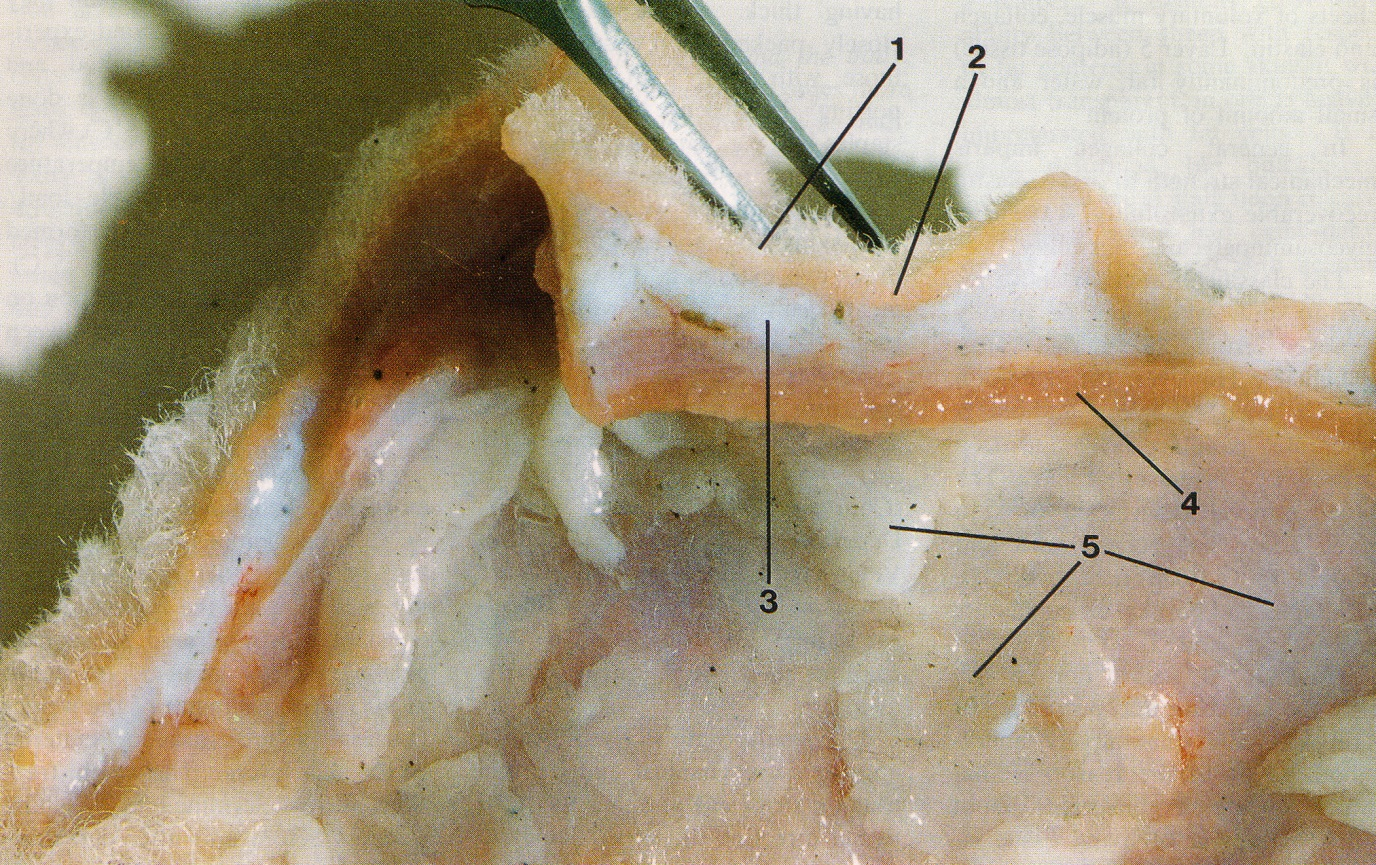
\includegraphics[width=1.0\textwidth]{sanazcollagenwrinkle-img1.jpg}
  \caption{Merino sheep skin showing layers. 1. epidermis with wool fibres; 2. papillary layer of dermis; 3. reticular layer of dermis; 4. areolar tissue and muscle; and 5. adipose tissue. Two wrinkles are present; one alongside each side of the forceps (from Mitchell et al (1984)~\cite{mitc:84})}
  \label{fig:mitchell}
\end{figure}

%\end{document}


Only the first 3 layers curve upward in a folded section of skin, layers 4 and 5 remain straight. This can be seen in Figure ~\ref{fig:mitchell}. Mitchell et al note that Layer2 is much weaker than Layer 3 ( collagen not as hard). When wrinkles or folds occur in the skin, Layers 1,2, and 3 buckle up into a fold, while Layers 4-5 are straight. It appears as if wrinkles are formed either by an overgrowth of Layers 1-3, or by a shrinkage or tightening of Layer 4. Mitchell has demonstrated this by showing that if Layer4 (and Layer 5) are dissected away from a skin specimen with wrinkles, the folds in Layers 1-3 flatten out. So in a wrinkled sheep, Layer 4 is holding the skin under some tension, which relaxes when Layer 4 is removed.

Even less is known about wrinkle development. Merino lambs are born with visible wrinkles.  A somewhat obsure reference (Bogolyubsky (1940)~\cite{bogo:40}) asserts that wrinkles were observed forming in foetal skin of Karakul and Merino lambs at around 100 days of gestation. That is about the time at which the secondary derived follicles initiate. Carter(1943)~\cite{cart:43} presents a photograph of the skin surface of a 10 day old Merino lamb (Plate 13 Figure 1) which clearly shows small {\em pin wrinkles}. There are no other studies of foetal wrinkle development, but there is a considerable literature on follicle development ( see Fraser and Short(1960)~\cite{fras:60} and Maddocks and Jackson(1988)~\cite{madd:88} and Ryder and Stevenson(1968)~\cite{ryde:68} for reviews). There is some literature on collagen development in sheep skin, and we will look at that below.

What is to be investigated in this study is that the amount and type ( and maybe timing and arrangement in the skin) of collagen development might be a factor involved with both wrinkle development and follicle development. So what is known about collagen? Well, it is already present in the dermis (layers 2 and 3) of foetal skin at the time follicles develop (Knight et al (1993) ~\cite{knig:93}). 
 These authors distinguish two collagen types ( Type III or 'soft' collagen, and Type I or 'hard' collagen) and note  that Type III is highest at 75 days of gestation, and falls progressively as the foetus develops, while Type I is low at day 75 and rises to over 50 percent by birth. Collagen fibres are formed from cells called {\em fibroblasts}. At 75-80 days the fibroblasts appear as plump, immature cells surrounded by reticular collagen fibres which are composed of Type III collagen. By birth the fibroblasts have matured  and the collagen fibres may be intermeshed to varying degrees. If the fine reticular fibre pattern remains, it is soft collagen, if the fibres intermesh the collagen tissue is hardened to various degrees. 

Collagen development, secondary follicle development and wrinkle formation  all seem to commence at the same time of around 100 days of foetal age.  Follicle development ceases at around birth ( 150 days) but development of collagen and wrinkles continues into the adult sheep. In this study we look at the end points of development - that is we study collagen and follicles in adult sheep with and without wrinkles. That will not reveal the details of development, but it should make clear any obvious associations between collagen, wrinkles, and follicles.

\section{Materials and Methods}
The experimental design was to choose, by visual inspection, individual sheep with wrinkle-free skin and wrinkly skin from each of a number of Australian Merino flocks. The flocks available for this study were mostly flocks which were undergoing breeding towards the SRS \textsuperscript{TM} Merino type. Consequently most of the sheep chosen as examples of wrinkle-free sheep would have the loose and supple skin which is characteristic of SRS \textsuperscript{TM} Merinos. There is another sort of wrinkle-free sheep which has low follicle density and tight skin and this type is probably not well represented in the present study.

Two trials were conducted
\begin{description}
\item[Trial 1]  Two sheep were chosen from each of six Merino flocks, one wrinkle-free and one wrinkles. This is a randomized block design without replication .  The blocks are the five flocks, and the treatment is the presence or absence of wrinkle.
\item[Trial 2]  Eighteen sheep were chosen from each of two flocks, nine wrinkle-free and nine with wrinkles. This is a randomised block design with replication. The second of these two flocks was more wrinkled and was not breeding towards the SRS \textsuperscript{TM} Merino type.
\end{description} 
\subsection{Skin samples}
In Trial 1 a biopsy sample was taken from the midside position on each sheep and the specimens were trimmed in the normal manner before processing, so that only Layer 1 (epidermis) and Layer 2 (papillary dermis) were present for histological observation.

In Trial 2 , for the sheep with wrinkly skins, skin biopsies were collected from on the wrinkles as well as between the wrinkles. For the wrinkle-free sheep only one biopsy sample was collected. These specimens included Layers 1 to 4, ie only the adipose tissue was trimmed.

Midside skin samples were collected using a 10 millimetre
circular trephine (Acu Punch® skin biopsy punches, Acuderm, Inc.) and
fixed in 10\% formol saline solution. 

\subsection{Macroscopic skin observations}

Skin samples were washed in several changes of water, the wool
stubble trimmed and then examined under a magnifying lamp ( x 3
magnification).  Scores for  suppleness (1 = hardened to 5 = supple)
of the papillary layer and reticular layer  were made.  Each skin
sample was examined to determine if layers 2 and 3, and layers 3 and 4,
were free or fixed and whether localized hardening and folding of the
skin had occurred.

The thicknesses of the papillary dermis and
the reticular dermis were measured using a ruler graduated in one
millimetre divisions. A Mitutoyo ballpoint gauge
(model no. 2046S) was then used to measure the compressed thickness at
four sites for each skin sample.

\subsection{Histological skin processing and observations}
\subsubsection{Collagen observations}

Skin samples used for haematoxylin and eosin staining (H-E) and
picrosirius red (PSR),were fixed in 10\% neutral buffered formalin for
24 hours before being processed to wax in an automated tissue
processing platform (Shandon Excelsior, Thermo Scientific, USA), and
then embedded in paraffin wax. Four micron sections were cut and placed
onto slides for H-E staining for tissue morphology. Serial section was
also employed on a separate slide for PSR staining to highlight
collagen content. Staining was performed manually.

Sections were then reviewed microscopically (BX53 Olympus, Australia)),
and images taken on 3 CCD camera (DP72, Olympus, Australia) under both
bright field and polarized conditions .

For PSR collagen analysis, the 40x objective was employed at a fixed
exposure to take high power images of 5 random deep dermal fields of
view for image analysis aimed at determining the amount of collagen in each field. 

The five images for each sample were then uploaded for quantitative analysis
via the ImagePro Plus (Media Cybernetics, USA) 7.1 software in which
thresholds were set to count all pixels comprising of the red staining
fibres in the PSR stained specimen field.  This provided a measure of the area of the field occupoed by red stained collagen fibres.

A slightly better measure of the total amount of collagen in the field could be obtained by allowing for the intensity of red staining of each pixel. This would be a measure density of collagen within the pixel and the depth of collagen through the thickness of the section.  The greyvalues for each pixel were converted to optical density, and the optical densities summed ( ie integrated) over all pixels in the field.
A mean was calculated for each specimen, averaged over 5 fields, and graphed.
The optical density data for each field subjected to analysis of variance to test for differences between wrinkle-free and wrinkled sheep, and , in Trial 2, to test for differences between on-wrinkle and between-wrinkle specimens within the wrinkled sheep.
All specimens were measured in this way, and this is one of the main quantitative results of the study.


Polarised light was employed in order to try and determine the type of
collagen present within each of the samples.
Collagen fibres stained with PSR have enhanced birefringency compared to that in H-E stained sections (Junqueira et al(1979)~\cite{junq:79}). Under polarised light they show coloured red,orange, yellow, or green, in order of thickness of the bundles of fibres. Thus red or orange would indicate Type I or hard collagen (which has thick bundles of fibres) while yellow or green would indicate Type III collagen which has individual fibres in a net-like structure.

Attempts to use polarised light images to make quantitative assesments of the amounts of each Type of collagen have been criticised in the literature (Lattouf et al (2014)~\cite{latt:14}).  The main issue seems to be that the birefringence is directional, only the fibres aligned with the direction of polarisation will show colours. We refrained from attempting this quantification, so our polarised light results are only qualitative.


\subsubsection{Vertical skin sections}
Vertical skin sections, approximately 0.3 millimetres wide, were cut
freehand with a sharp razor blade on a freezing stage and stained with
0.25 \% Nile blue sulphate, as described by Nay (1973).
The sections were cut parallel with the angle of
emergence of the fibres to avoid cutting through follicles. Mean
follicle curvature was scored from 1 = straight follicles to 7 =
tangled follicles by reference to a set of standard drawings used by
Nay and Johnson (1973). Follicle depth was measured
as both the perpendicular and angular distances (in millimetres)
between the skin surface and the lower ends of the follicle bulbs,
along with follicle bending, as described by Maddocks and Jackson
(1988).


\subsubsection{Horizontal skin sections}
Horizontal skin sections were also prepared as described by
Maddocks and Jackson (1988) using the frozen section technique and
measurement procedures of Nay (1973). The sections were used to measure
follicle density, secondary follicle to primary follicle ratio (S/P
ratio), primary fibre diameter and secondary fibre diameter of the
sheep.

JW to describe measurement of orientation of follicle groups
and measurements made of collagen sheets in subfollicular layer of
papillary dermis.


\subsection{Summary of measurements}


\subsection{Statistical Methods}

Data were imported into the R statistical program~\cite{rprog:13} and analysed using the {\em aov()} function for analysis of variance.
Allowance was made for the subsampling design by choosing  an appropriate error level for the F tests in analysis of variance. 

\section{Results}
We follow the path of looking first at overall morphology of skin specimens, then at the details of collagen structure, and finally at other related measurements

\subsection{Macro observations on biopsy specimen}
In Table~\ref{tab:macro} we present the suppleness scores and percent compressibility of specimens from the sheep from Trial 1.
%\documentclass{article}
%\usepackage{lscape}
%\begin{document}

\begin{table}[htp]
\centering
\caption{Suppleness scores and compressibility measurements for Flocks 1 to 5 of Trial 1}
\label{tab:macro}
\vspace{0.1in}
\begin{tabular}{|p{0.6in}|p{0.6in}|p{0.8in}|p{0.8in}|p{0.9in}|}  \hline
     Flock No. & Sheep No.  &  Skin Type & Suppleness Score & Compressibility Percent \\ 
\hline
  1 & W206 & Wrinkle-free & 5 & 75 \\
  1 & W205 & Wrinkled     & 2 & 54 \\
  2 & W490 & Wrinkle-free & 5 & 64 \\
  2 & W479 & Wrinkled     & 2 & 39 \\
  3 & W555 & Wrinkle-free & 5 & 67 \\
  3 & W547 & Wrinkled     & 1 & 58 \\
  4 & W567 & Wrinkle-free & 5 & 70 \\
  4 & S558 & Wrinkled     & 2 & 63 \\
  5 & Z529 & Wrinkle-free &   &    \\
  5 & Z530 & Wrinkled     &   &    \\
  5 & S283 & Wrinkle-free & 5 & 69 \\
  5 & W290 & Wrinkled     & 2 & 44 \\ \hline
\end{tabular}
\end{table}

%\end{document}

We see that the wrinkled sheep specimens were consistently less supple and less compressible than those of the wrinkle-free sheep.
These differences in Suppleness and Compressibility were tested for significance in an analysis of variance shown in Table~\ref{tab:macrot1aov}
% latex table generated in R 3.4.2 by xtable 1.8-2 package
% Fri Jul  5 17:48:54 2019
\begin{table}[ht]
\centering
\caption{Analysis of variance of Suppleness score and Compressibility}
\label{tab:macrot1aov}
\vspace{0.1in}

\begin{tabular}{lrrrrr}
 & Response Suppleness & & & \\
  \hline
 & Df & Sum Sq & Mean Sq & F value & Pr($>$F) \\ 
  \hline
FlockNo     & 1 & 0.00 & 0.00 & 0.00 & 1.0000 \\ 
  SkinType    & 1 & 25.60 & 25.60 & 224.00 & 0.0000 \\ 
  Residuals   & 7 & 0.80 & 0.11 &  &  \\ 
   \hline
\\
 & Response Compressibility & & & \\
  \hline
 & Df & Sum Sq & Mean Sq & F value & Pr($>$F) \\ 
  \hline
FlockNo & 1 & 0.20 & 0.20 & 0.00 & 0.9575 \\ 
  SkinType & 1 & 756.90 & 756.90 & 11.54 & 0.0115 \\ 
  Residuals & 7 & 459.00 & 65.57 &  &  \\ 
   \hline
\end{tabular}
\end{table}


The differences between skin types ( wrinkled and wrinkle-free) were significaant for both Suppleness and Compressibility. Flock differences were not significant.

\subsection{Skin tissue Morphology}
The pairs of wrinkle free and wrinkled sheep from each flock in Trial 1 showed consistent visual differences in their tissue structure. Figure~\ref{fig:trial24xhe} shows vertical sections stained with H-E from the wrinkled and wrinkle-free pair of sheep from flock 2.

%\documentclass{article}
%\usepackage{graphicx,subfigure}
%\usepackage{caption,rotating}
%\begin{document}

\begin{figure}[p]
\centering
 \subfigure[Plate (i) Sheep 3437 Wrinkled]{
    \label{fig:trial1he(i)}
    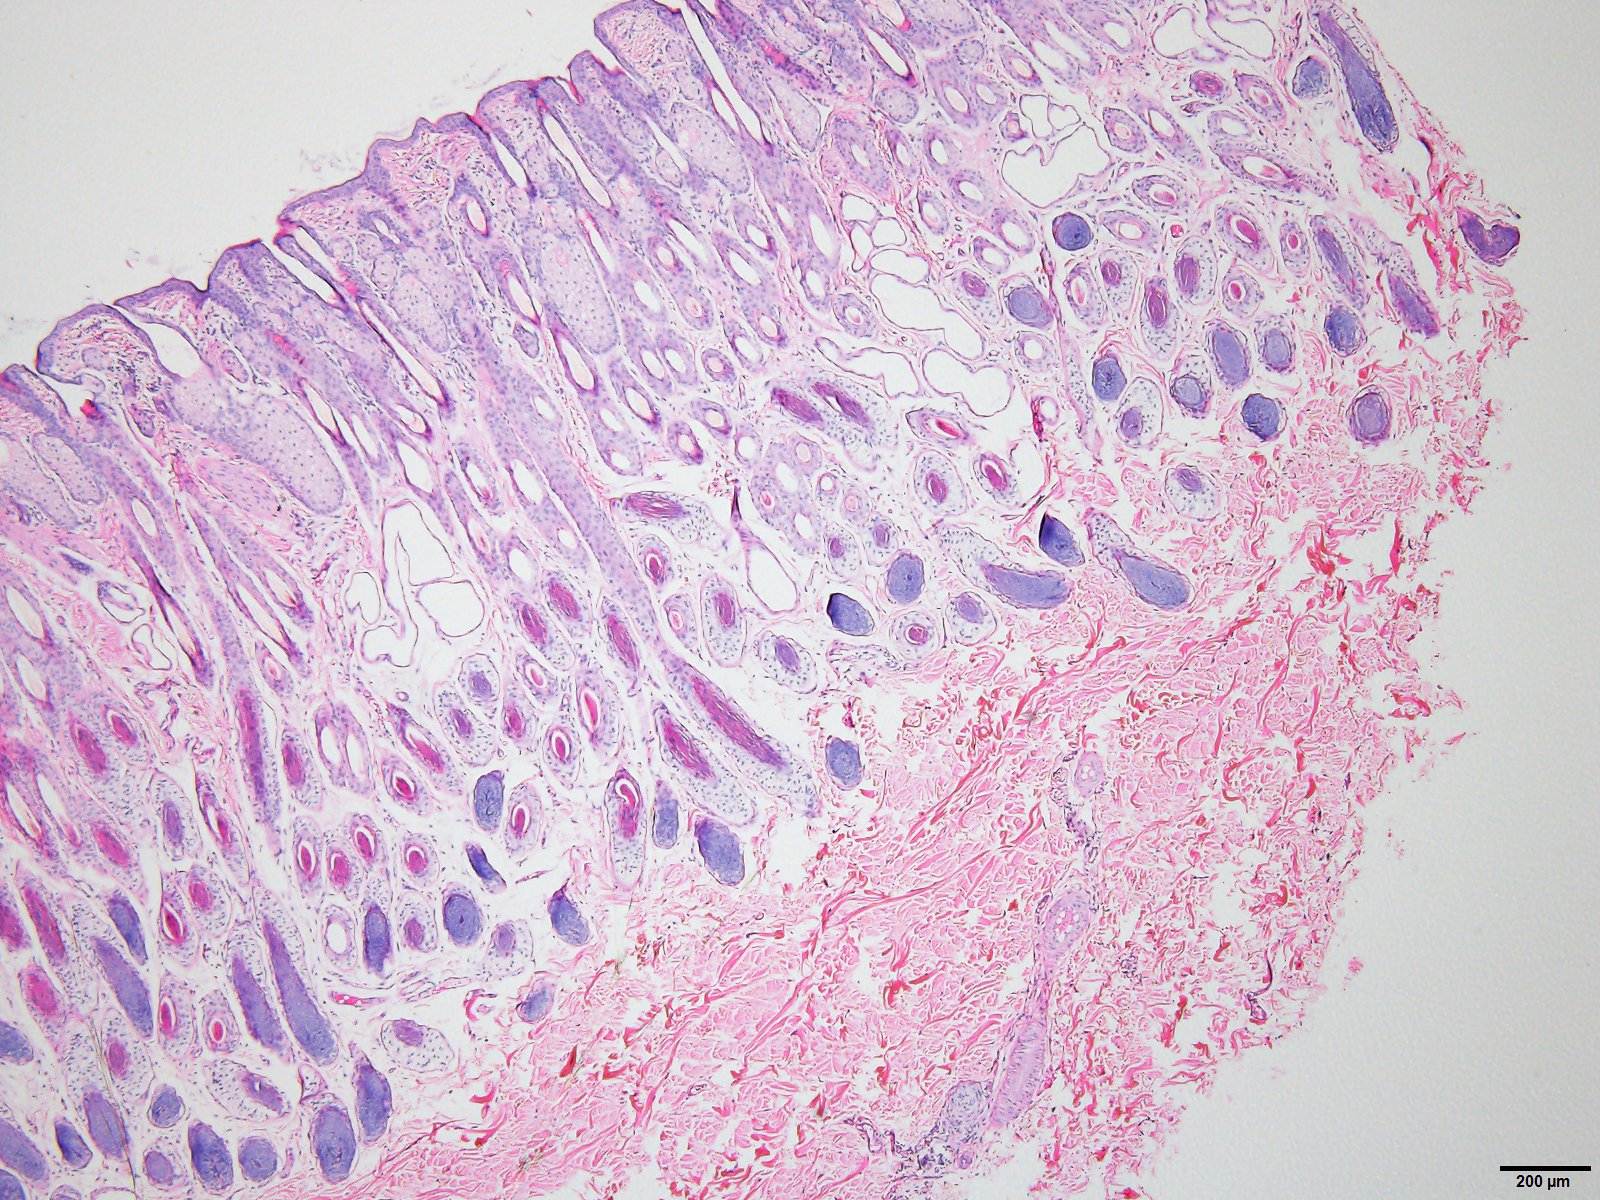
\includegraphics[scale=0.20]{3437_on_wrinkle_4x.jpg}
% 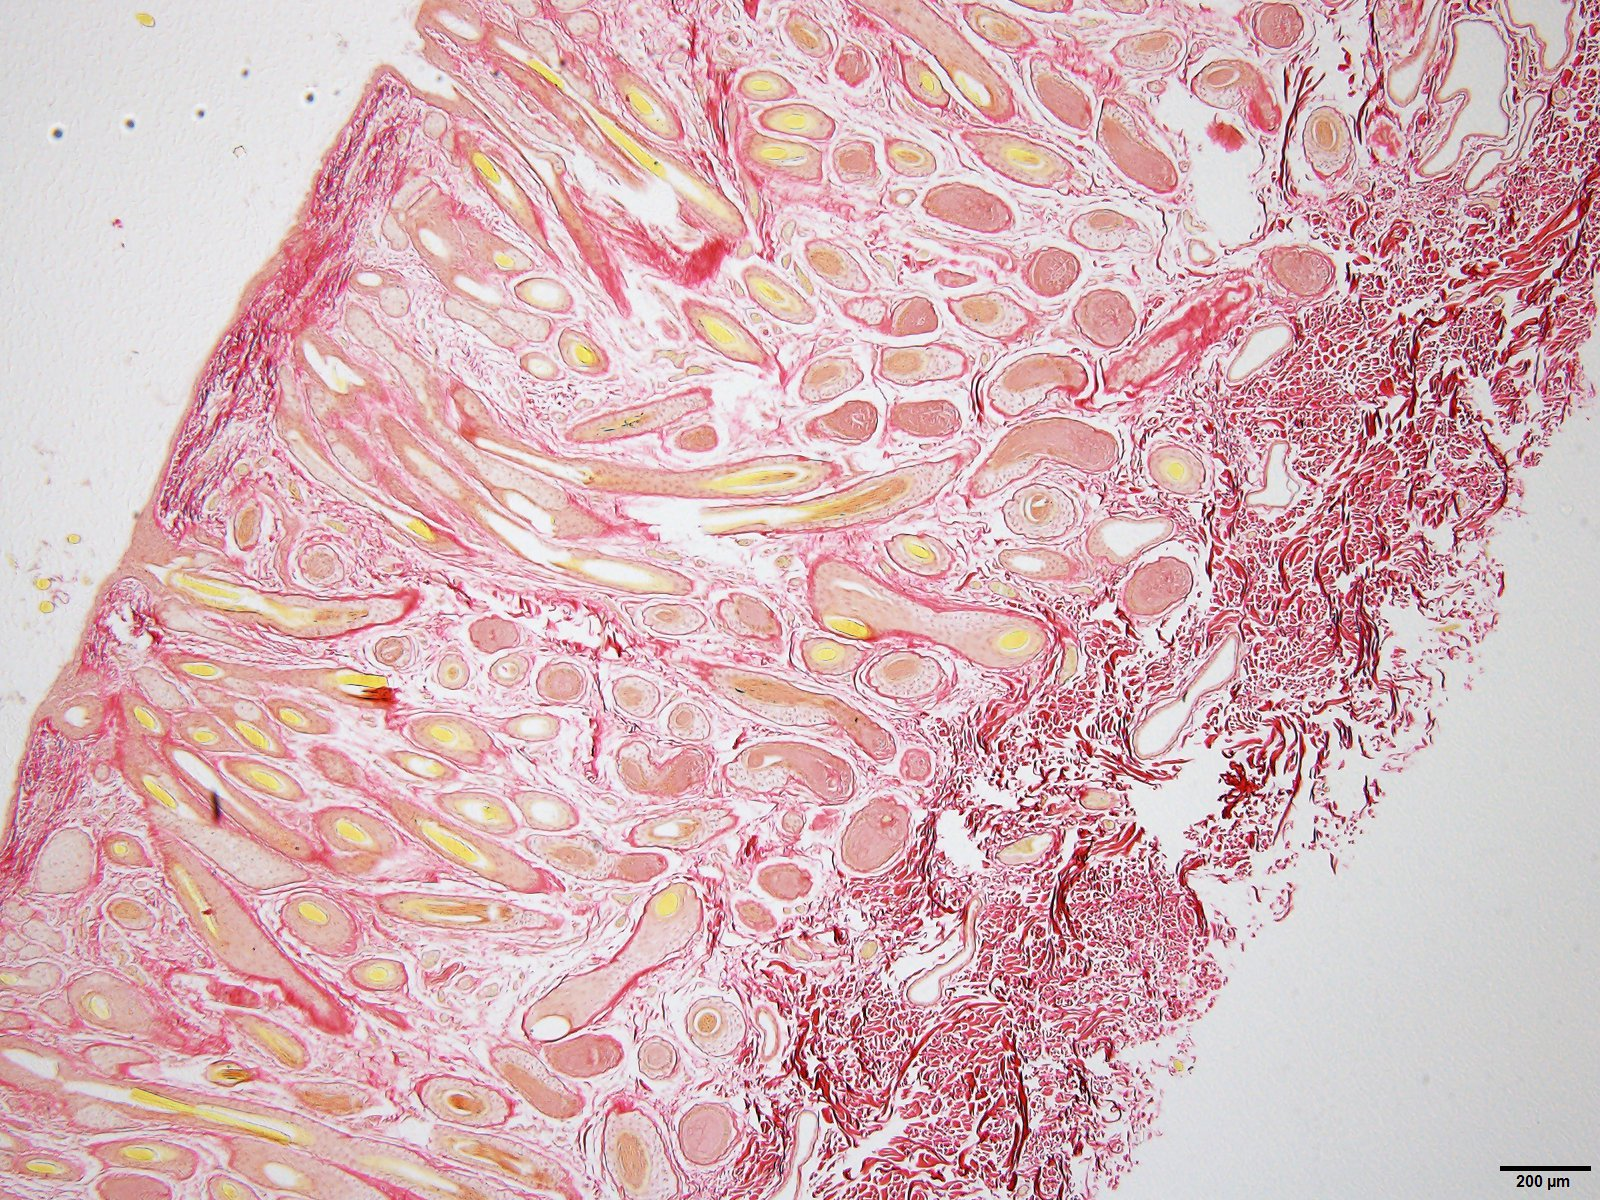
\includegraphics[width=1.0\textwidth]{w479-2-rigid.jpg}
  }
 \subfigure[Plate (ii) Sheep 3457 Wrinkle-free]{
    \label{fig:trial1he(ii)}
    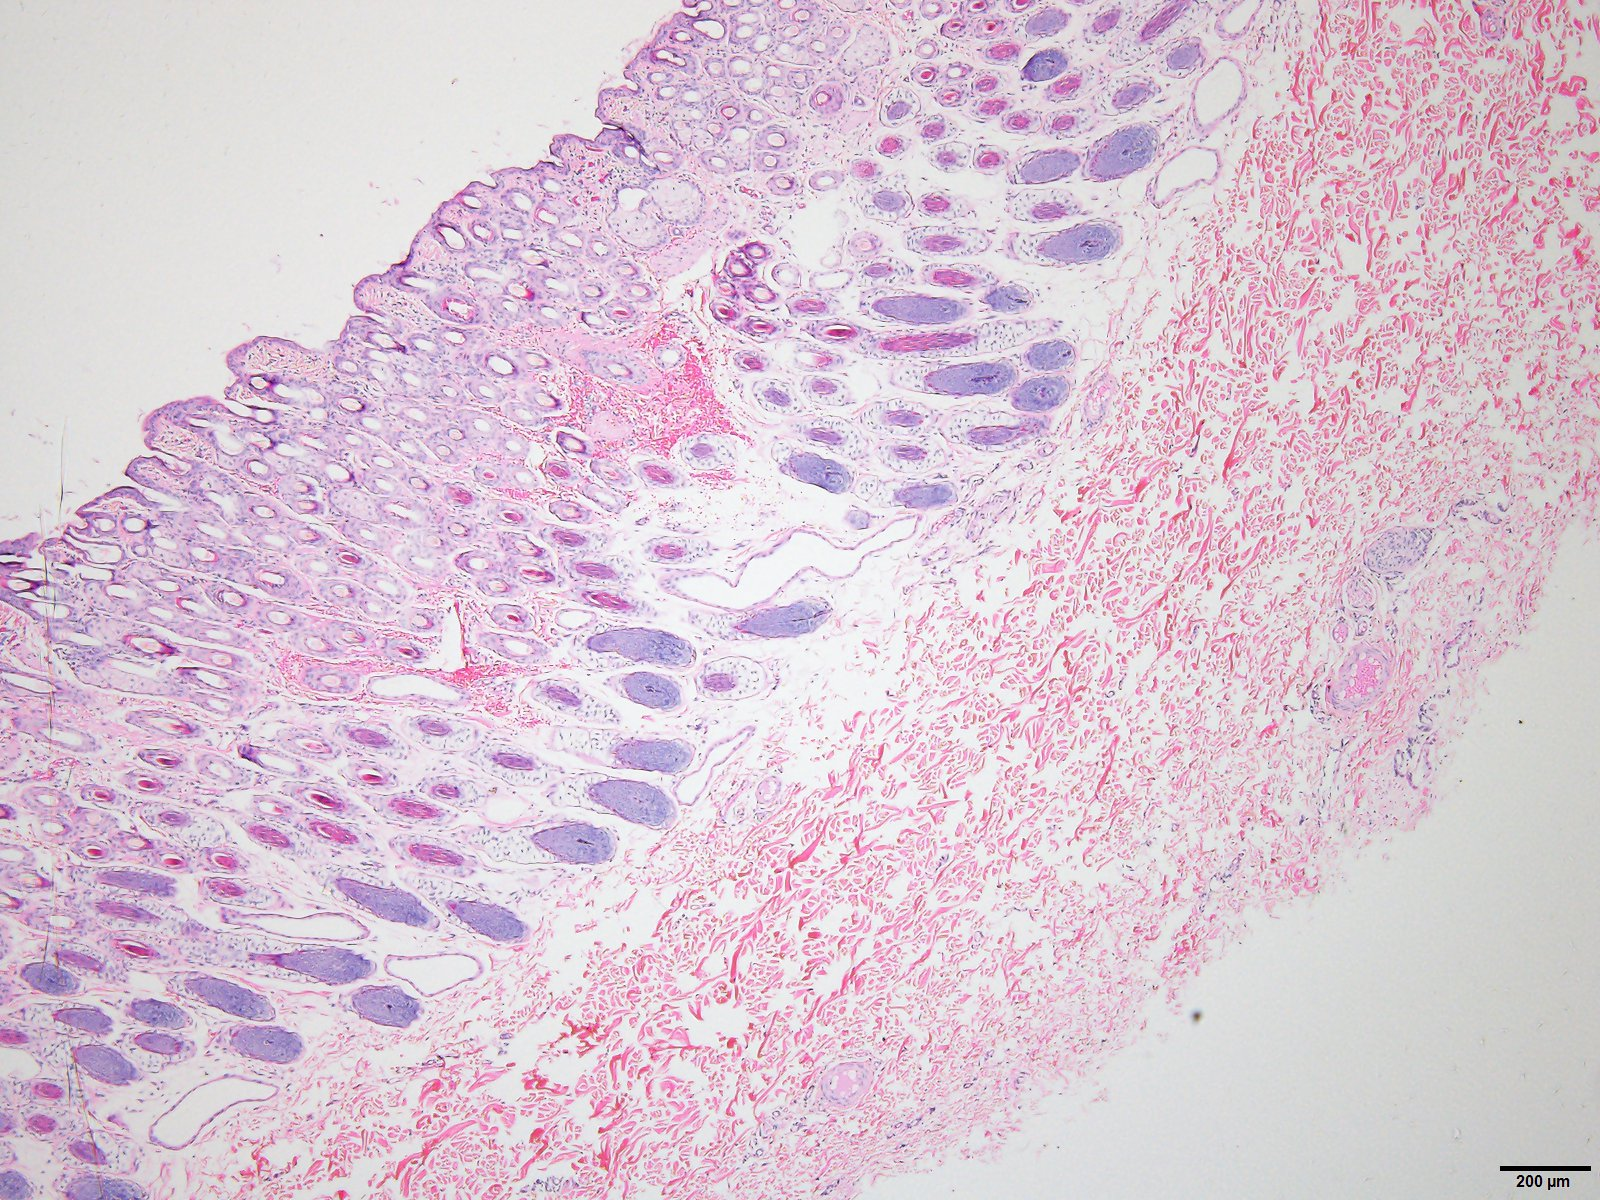
\includegraphics[scale=0.20]{JW_3457_smooth_4x.jpg}
  }
  \caption{Vertical sections from a wrinkled (i) and a wrinkle-free (ii)  sheep from Trial 2 flock 1 stained with H-E. }
\vfill
  \label{fig:trial24xhe}
\end{figure}

%\end{document}



The wrinkled sheep has a greater amount of staining in the  connective tissue in the lower dermis below the deepest follicle bulbs and to some extent in between the deepest bulbs. The staining also seems to be in larger clumps in the wrinkled sheep, whereas in the wrinkle-free sheep the lower dermal connective tissue has a finer more regular structure. 

  The follicles in the wrinkled sheep are at a variety of angles and are curved, as evidenced by the follicle shafts being sectioned and the follicle bulb being elliptical indicating sectioning at an angle. In contrast in the wrinkle-free sheep the sectioned follicles are more uniform. 

These differences were consistent across all sheep.

Although the Trial 2 biopsy samples were not trimmed before sectioning, the specimens displayed in Figure~\ref{fig:trial24xhe} do not show any layers below Layer 3. We need to see what connective tissue is present in Layer 4 (muscle layer). 
\begin{verbatim}
Sanaz, do you know why these sections have Layer 4 trimmed ? 
They are from Trial 2, and should be untrimmed.
The only images of untrimmed samples that I could find were the two below
 which came to me from Jim by email. There are none in his computer files
 which Sally retrieved for me?
\end{verbatim}

  We can check on this by looking at a specimen , which was not trimmed before sectioning. Figure~\ref{fig:trial2he} shows one example section which is from a wrinkled sheep from Flock 1 of Trial 2.
%\documentclass{article}
%\usepackage{graphicx,subfigure}
%\begin{document}

\begin{figure}[!h]
  \centering
  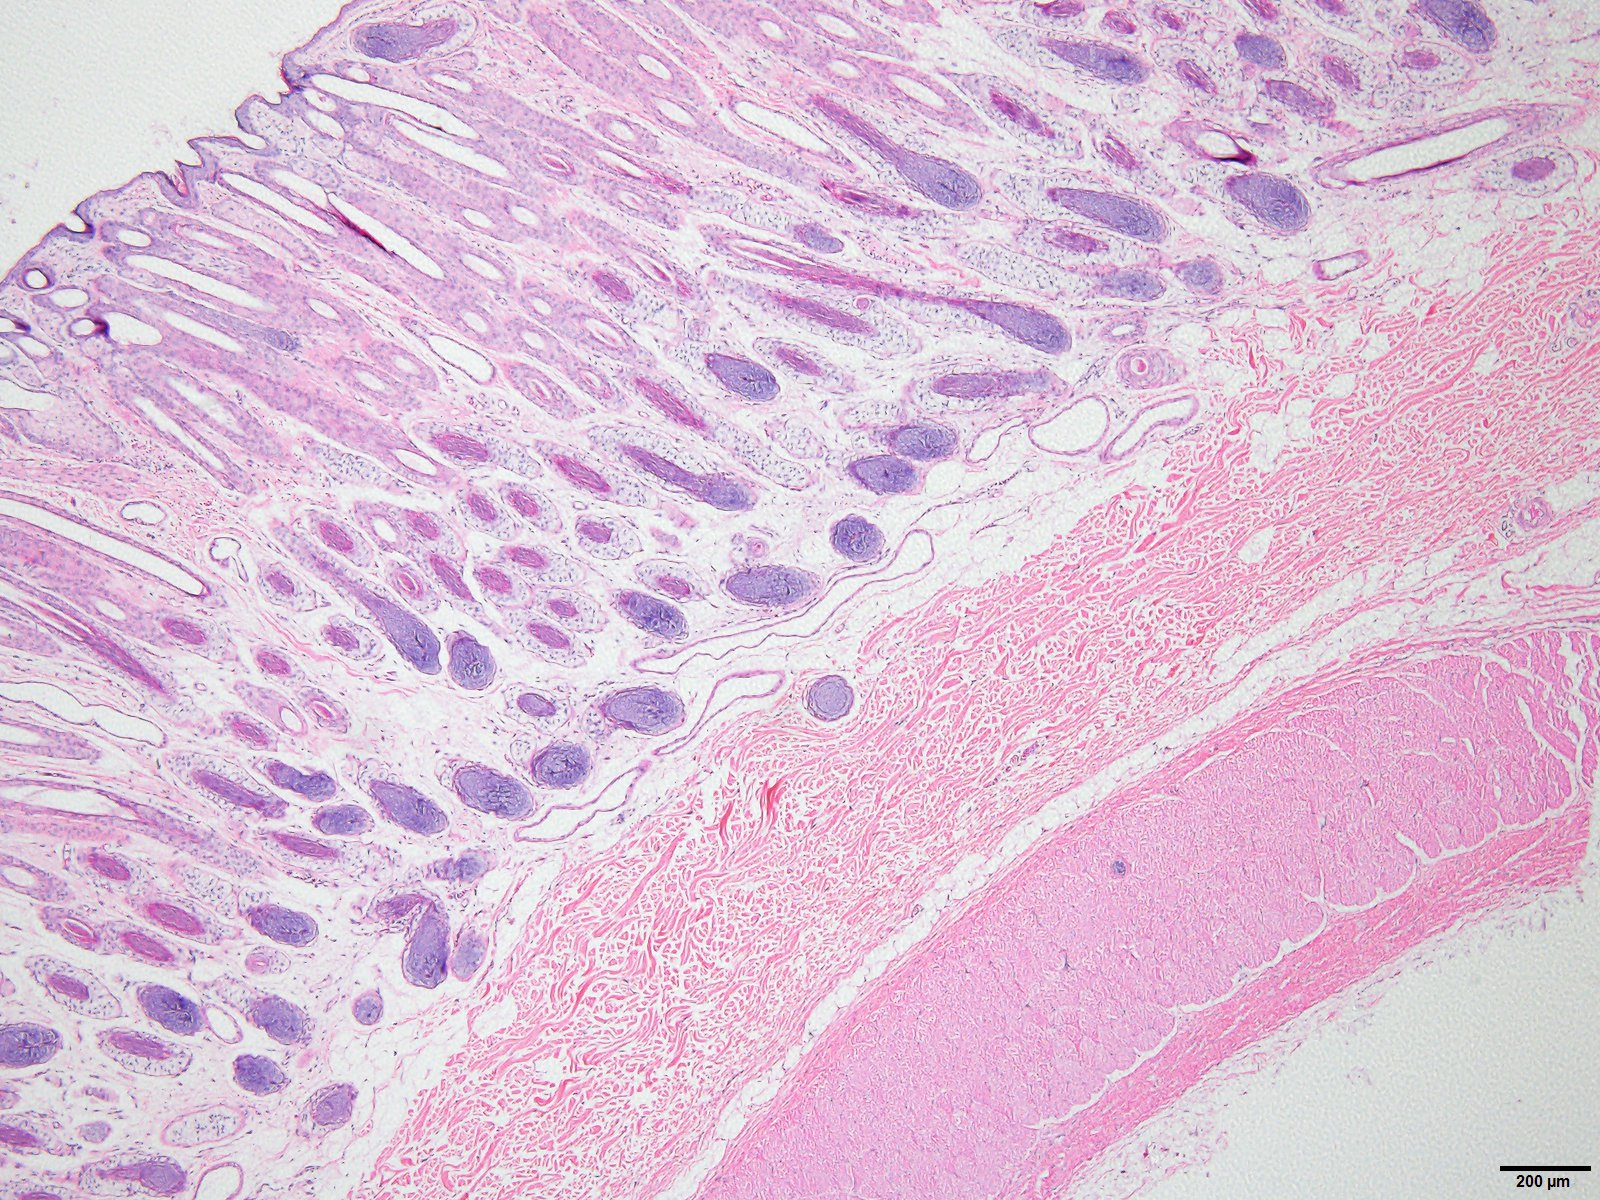
\includegraphics[width=1.0\textwidth]{3456_4layers_4x.jpg}
  \caption{Vertical section from a wrinkled sheep (3456) from Trial 2 Flock 1 stained with H-E. This section is from an untrimmed biopsy specimen and shows all 5 layers (Epidermis, Papillary dermis, Reticular dermis, Areolar tissue and Muscle layer, and Adipose tissue).}
  \label{fig:trial2he}
\end{figure}

%\end{document}



It is clear from Figure~\ref{fig:trial2he} that there is connective tissue in Layer 3 (lower or reticular dermis), then a layer which may be muscle and/or connective tissue, then a wider layer of adipose tissue, and finally another layer of muscle and/or connective tissue.  The muscle layer(s) have only stained with the pink eosin counterstain and do not show the reticular structure of  connective tissue. 

We are concerned with the nature of the connective tissue in the lower dermis only. We wish to quantify and qualify the way in which it differs between wrinkled and wrinkle-free sheep.

\subsection{Detailed morphology of connective tissue} 
The stain picrosirius red (PSR) was used to differentiate collagen from other components of connective tissue. Figure~\ref{fig:trial2psr} shows a section from the same sheep as Figure~\ref{fig:trial2he} examined with normal bright field microscopy. 
%\documentclass{article}
%\usepackage{graphicx,subfigure}
%\begin{document}

\begin{figure}[!h]
  \centering
  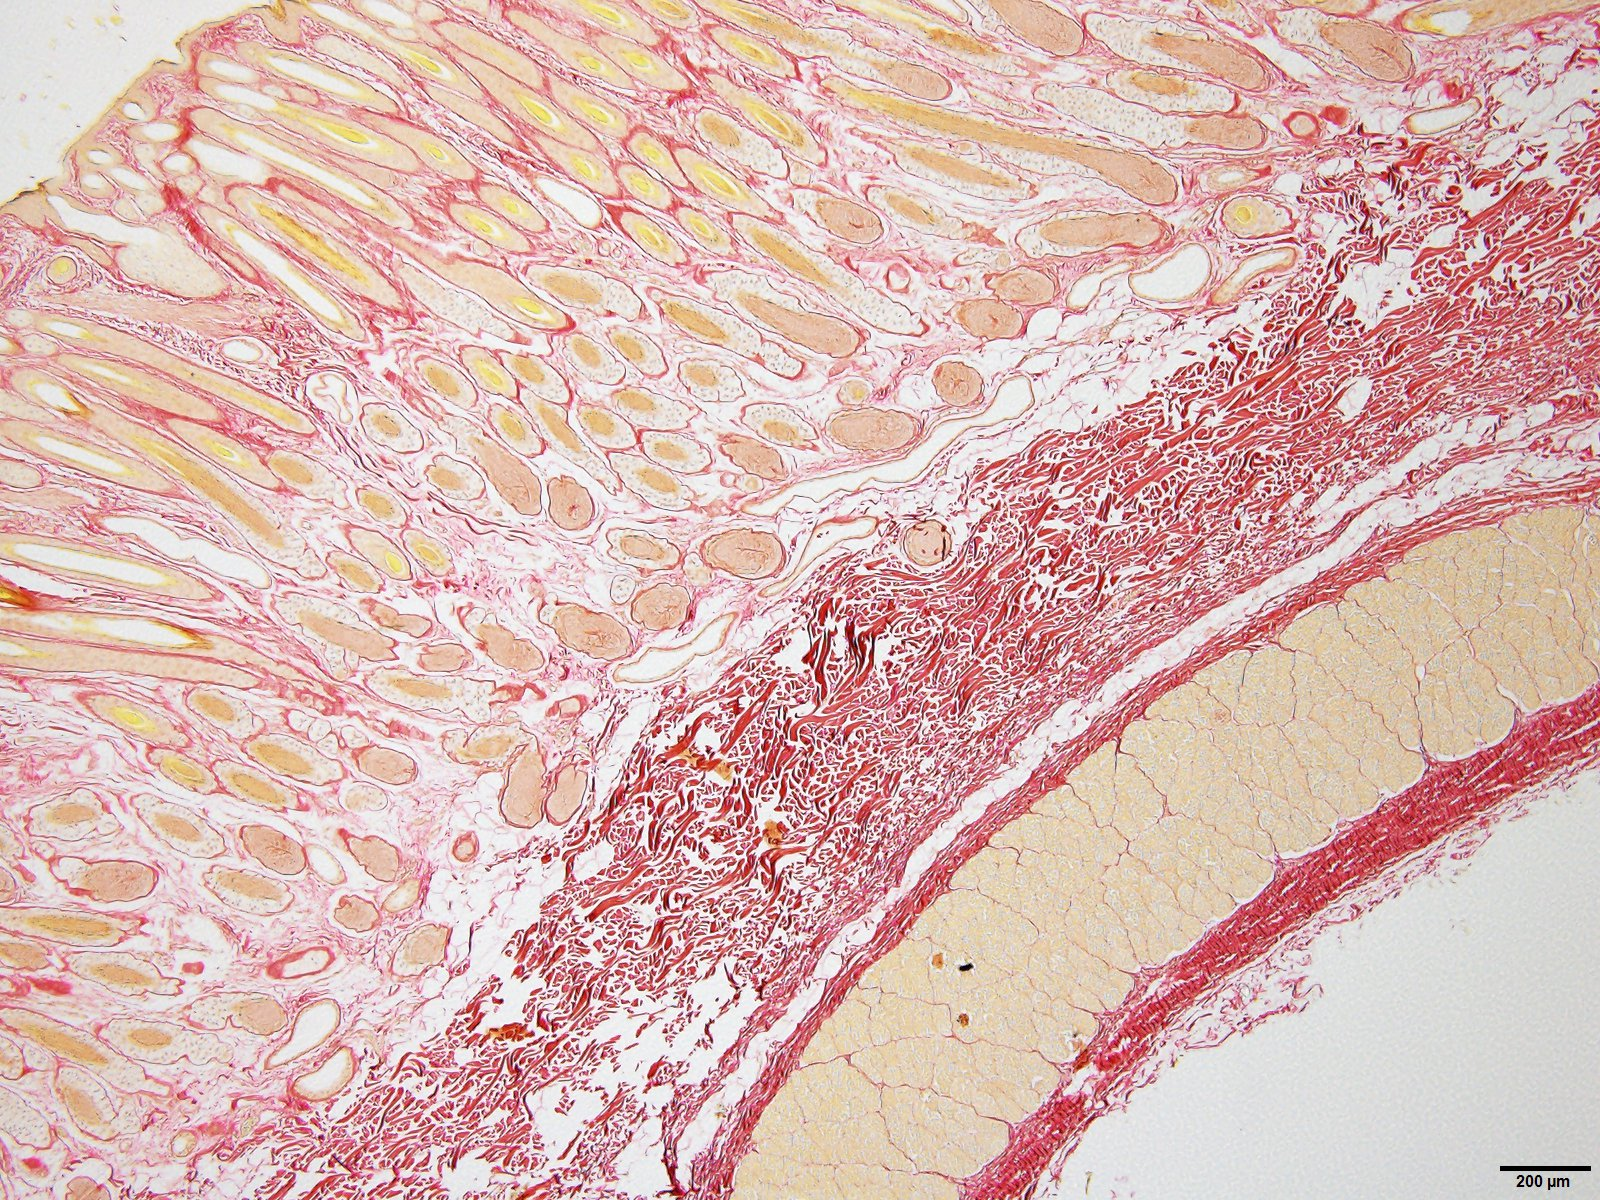
\includegraphics[width=1.0\textwidth]{3456_4layers_4x_PSR.jpg}
  \caption{Vertical section from a wrinkled sheep (3456) from Trial 2 Flock 1 stained with PSR and viewed with bright field microscope. This section is from an untrimmed biopsy specimen and shows all 5 layers (Epidermis, Papillary dermis, Reticular dermis and the Fat/Muscle layers). Collagen (stained red) is present in Layers 2 and 3, and on the borders of the Adipose layer}
  \label{fig:trial2psr}
\end{figure}

%\end{document}


The collagen is stained red. There is some collagen showing in the Layer 2 (papillary dermis), a dense band of collagen in Layer 3 (subpapillary dermis), and Layers 4 and 5 consist of yellow stained adipose tissue with a band of dense red collagen above and below it. These two bands are muscle tissuea which contains both collagen and elastin fibrils.  Wool fibres and follicle bulbs are stained yellow by the picric acid component of PSR. Within the  adipose tissue layer there are tiny tracks of red stained connective tissue, presumably between the fat cells.

So we can conclude that the  connective tissue in Layer 3 of wrinkled sheep contains collagen. 

\subsubsection{Amount of collagen}
Since the nature of the connective tissue in Layer 3 is what seems to differ between wrinkled and wrinkle-free sheep, we attempt to quantify the difference in amount of collagen to see if this explains the observed difference in appearance.

To quantify the amount of collagen in Layer 3, 5 fields under a 40x objective were chosen at random from within Layer 3 (reticular dermis) of each PSR stained section from each sheep in Trials 1 and 2. A typical image from one field of a wrinkled and a wrinke-free sheep is shown in Figure~\ref{fig:psr40x}.
%\documentclass{article}
%\usepackage{graphicx,subfigure}
%\usepackage{caption,rotating}
%\begin{document}

\begin{figure}[p]
\centering
 \subfigure[Plate (i) Sheep 3437 Wrinkled]{
    \label{fig:trial1he(i)}
    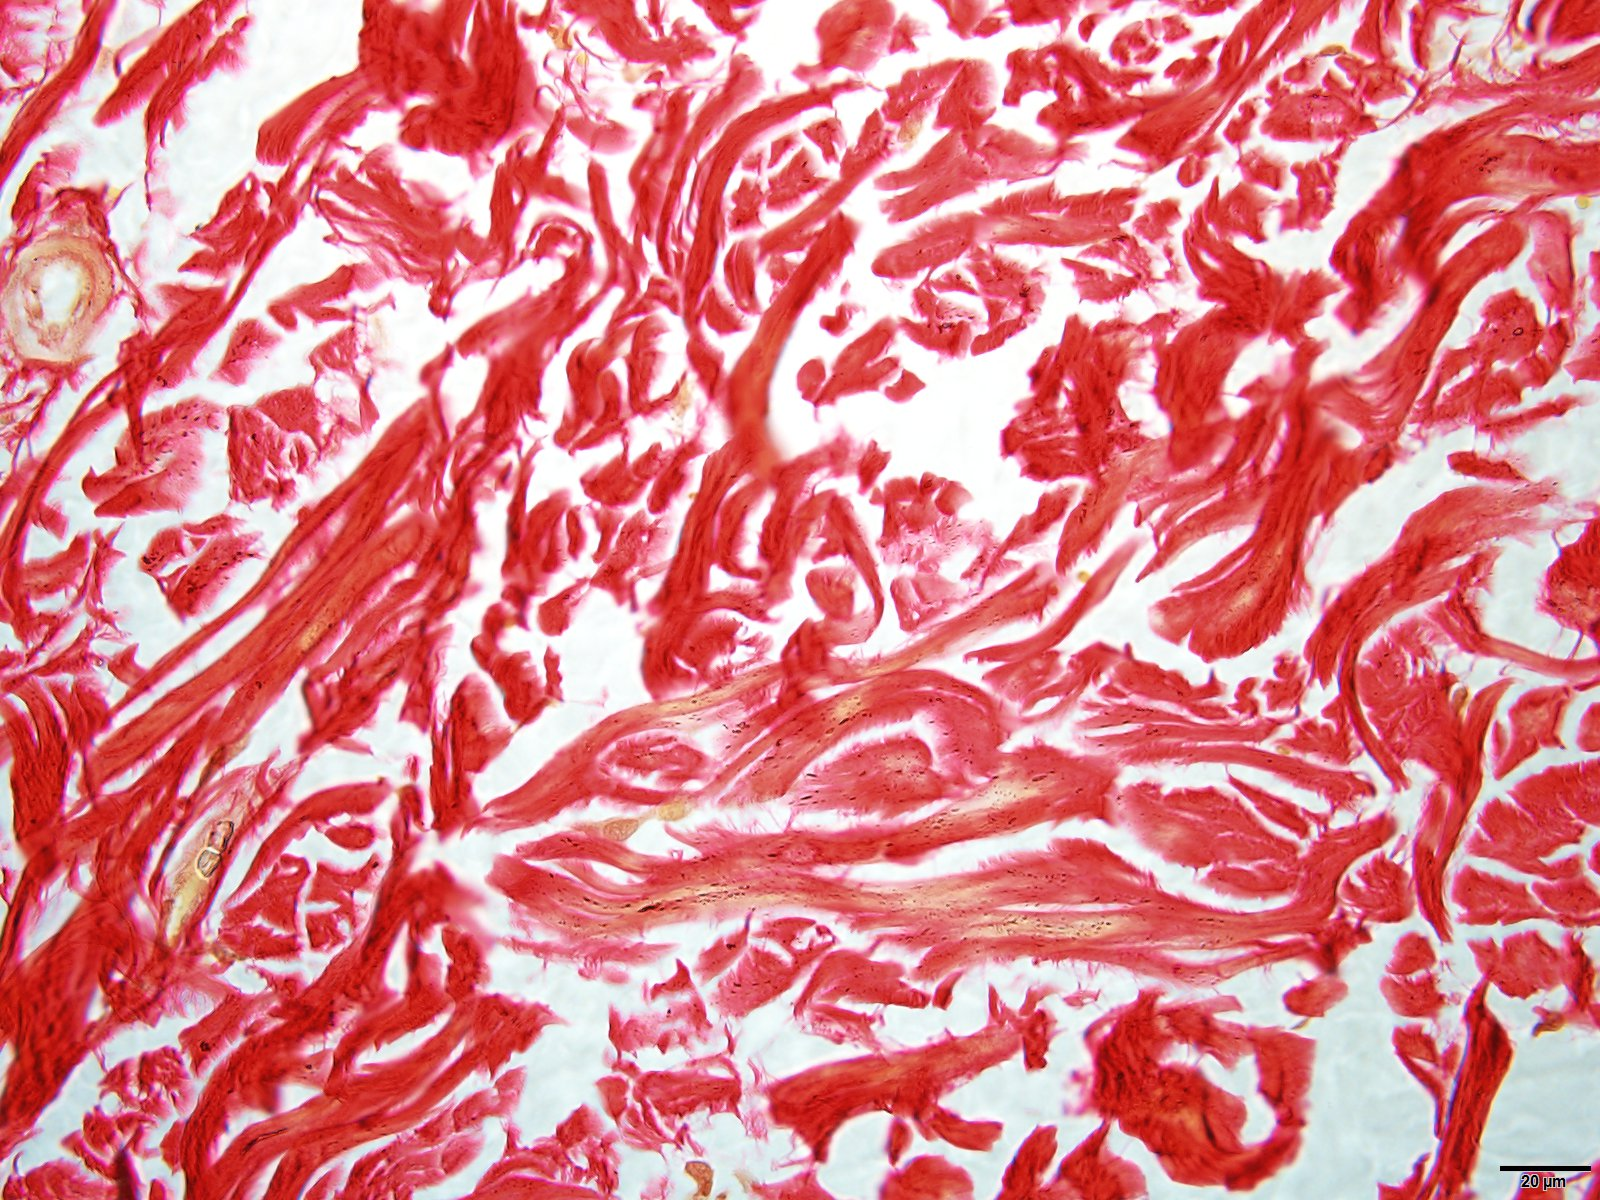
\includegraphics[scale=0.20]{3437_on_wrinkle_1.jpg}
% 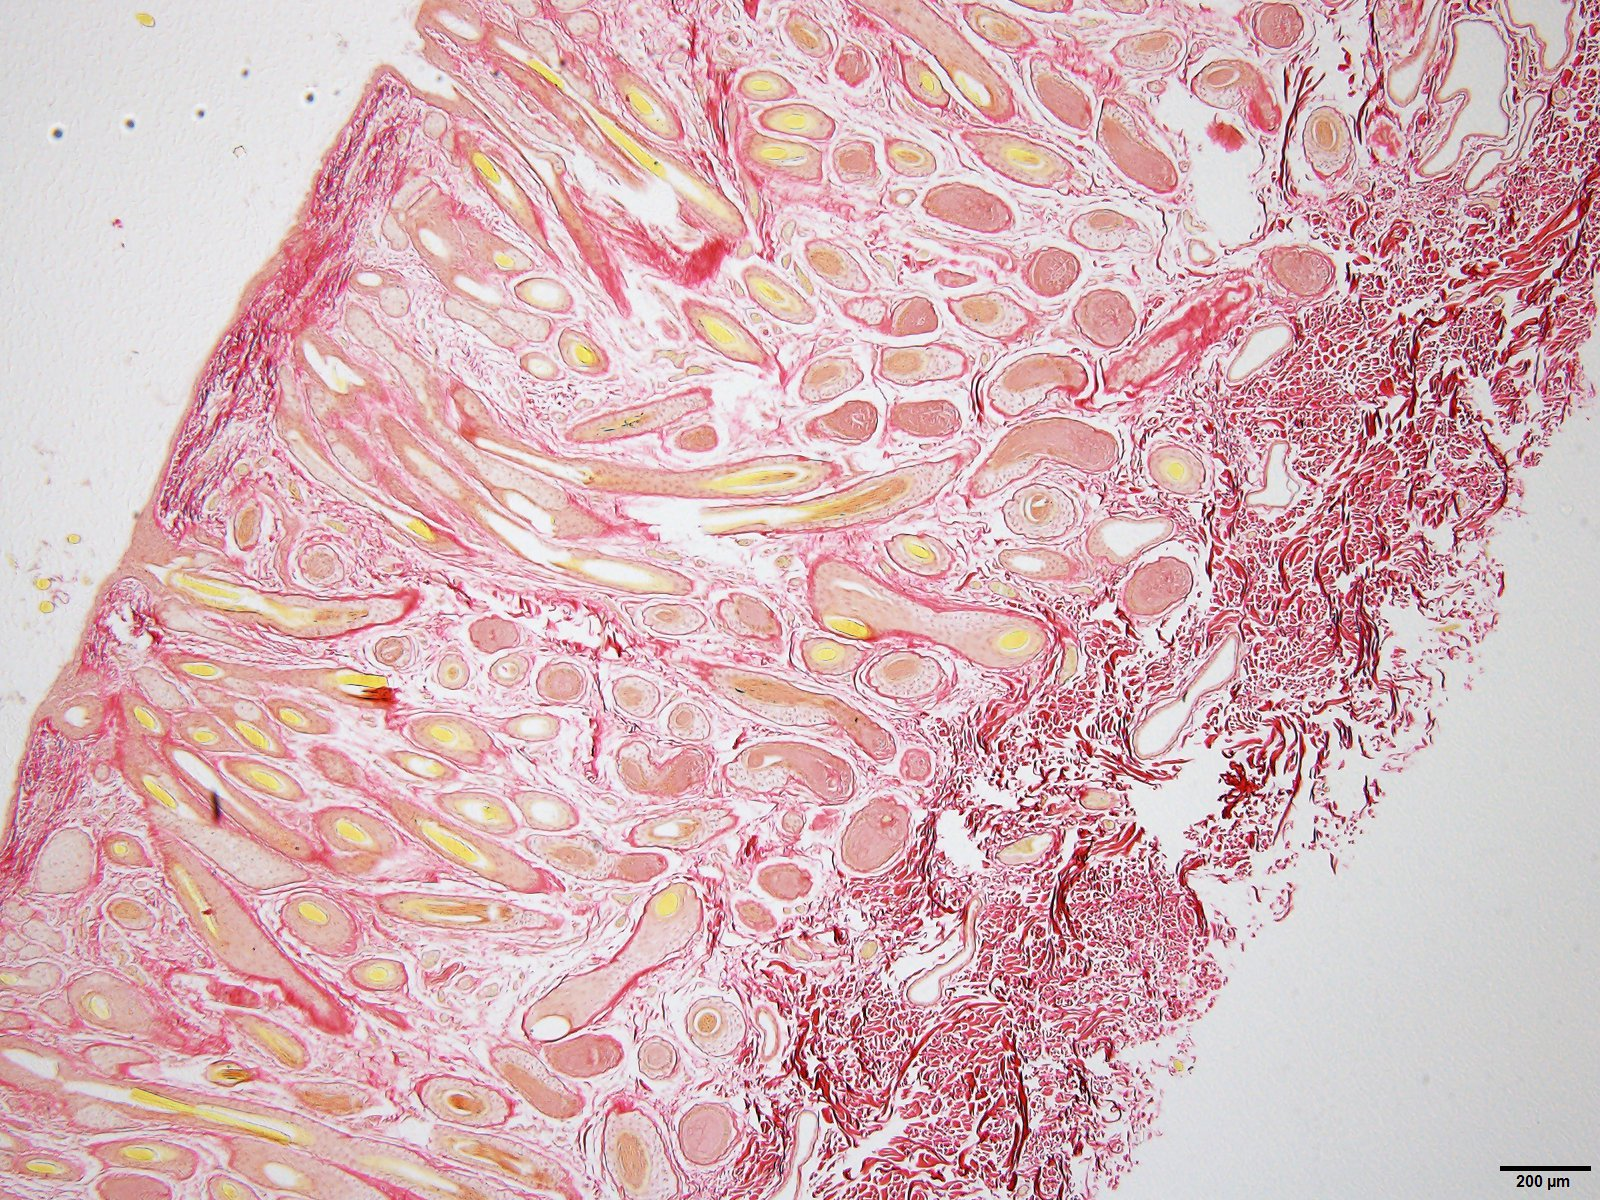
\includegraphics[width=1.0\textwidth]{w479-2-rigid.jpg}
  }
 \subfigure[Plate (ii) Sheep 3457 Wrinkle-free]{
    \label{fig:trial1he(ii)}
    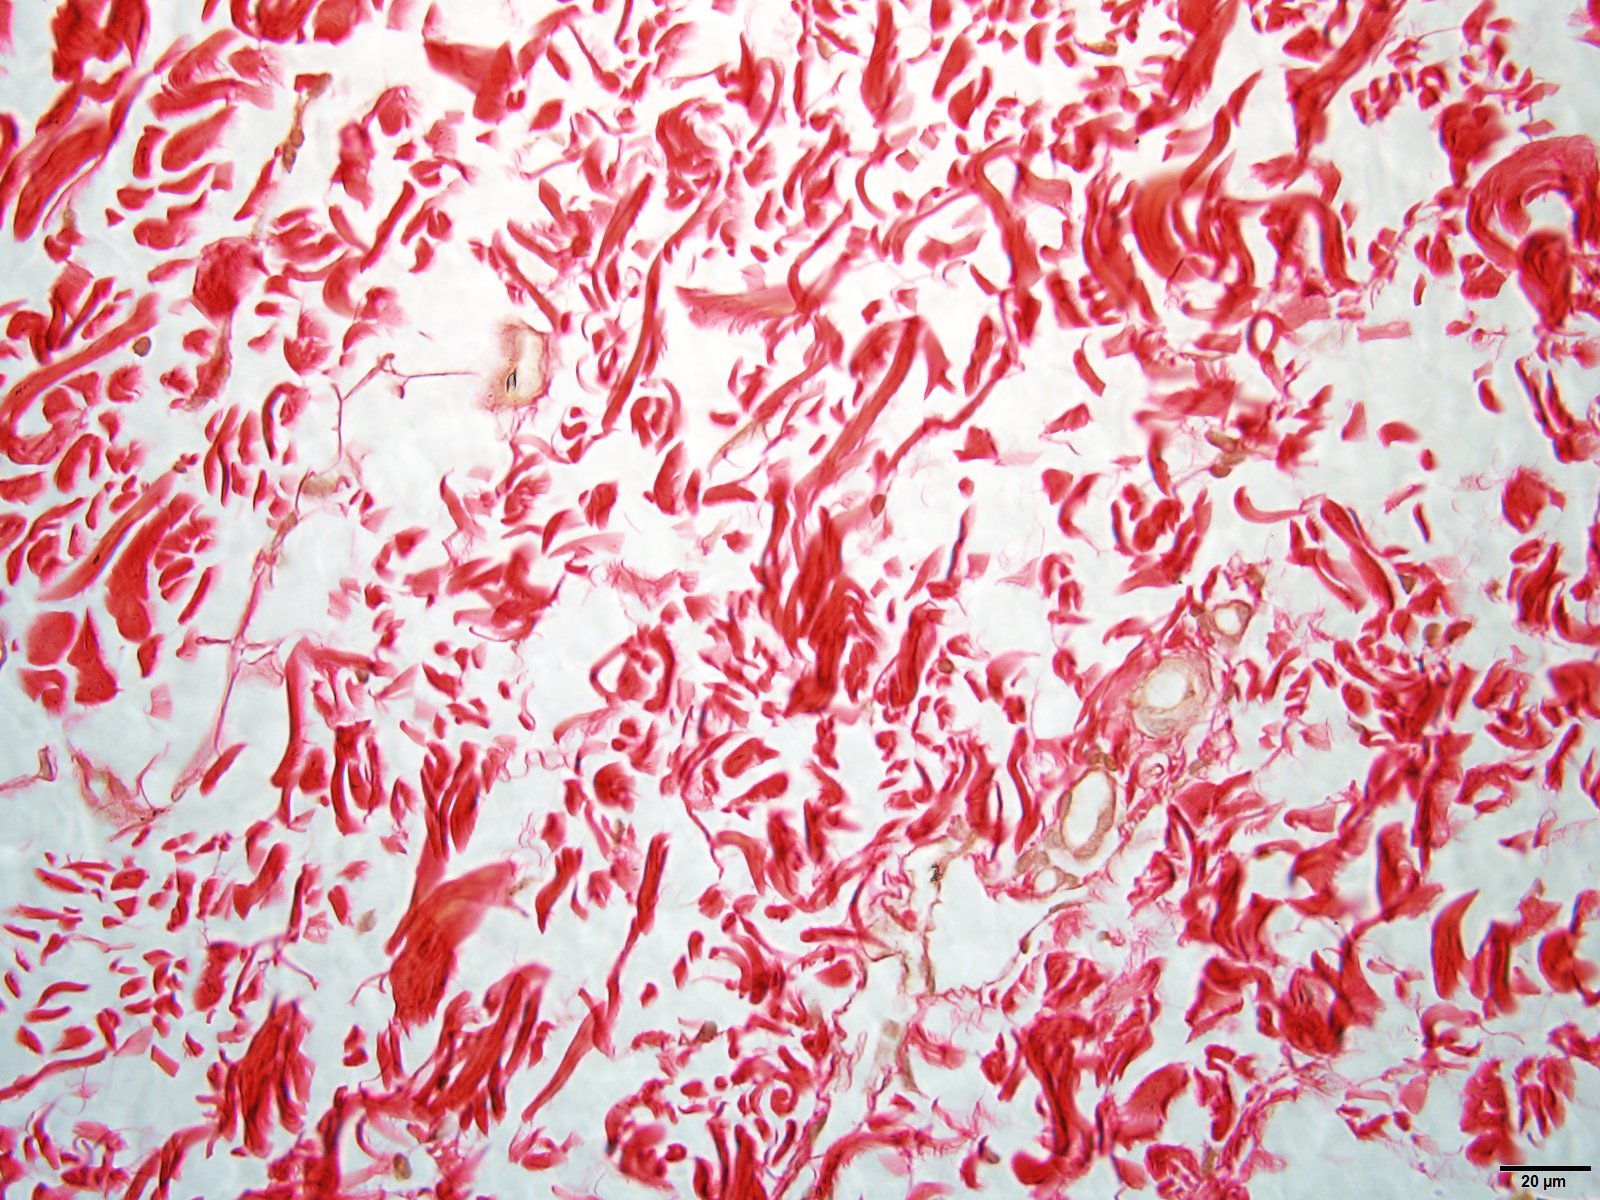
\includegraphics[scale=0.20]{3457_smooth_3.jpg}
  }
  \caption{Fields chosen at random from within Layer 3 (subpapillary dermis) stained with PSR and viewed with a 40x objective.}
\vfill
  \label{fig:psr40x}
\end{figure}

%\end{document}


The two fields shown in Figure~\ref{fig:psr40x} were chosen to be typical of the difference between wrinkled and wrinkle-free sheep. They show that the collagen in Layer 3 of wrinkled sheep is in larger aggregates (bundles of collagen fibres), and suggest that there is more collagen present ( as evidenced by more red stained areas) in wrinkled sheep. We set out to confirm this with some quantitative data.

 The image analysis procedure described in the methods was used to assess the total amount of red stained pixels in each field.  What was actually calculated was the sum of the calibrated optical densities of all the pixels in the red image. The integrated (ie summed over all pixels) red pixel optical density for each sheep is shown  in Figure~\ref{fig:redpixt1} for Trial 1 and Figure~\ref{fig:redpixt2} for Trial 2.
%\documentclass{article}
%\usepackage{graphicx,subfigure}
%\begin{document}

\begin{figure}[!h]
  \centering
  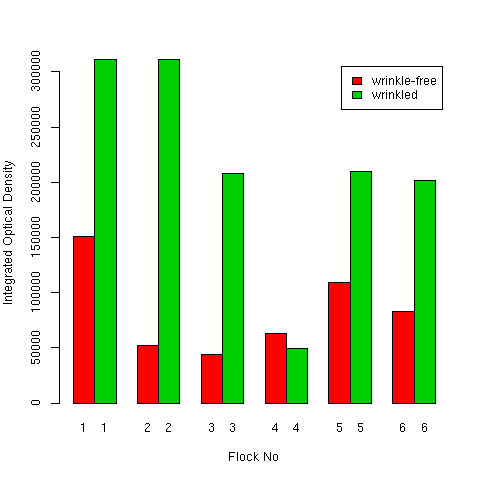
\includegraphics[width=0.8\textwidth]{t1odmeans.png}
  \caption{Integrated optical density of the red images of sections stained with PSR for each sheep in Trial 1 averaged over five microscope fields}
  \label{fig:redpixt1}
\end{figure}

%\end{document}


%\documentclass{article}
%\usepackage{graphicx,subfigure}
%\usepackage{caption,rotating}
%\begin{document}

\begin{figure}[p]
\centering
 \subfigure[Plate (i) Flock No 1 of Trial 2]{
    \label{fig:redpixt2(i)}
    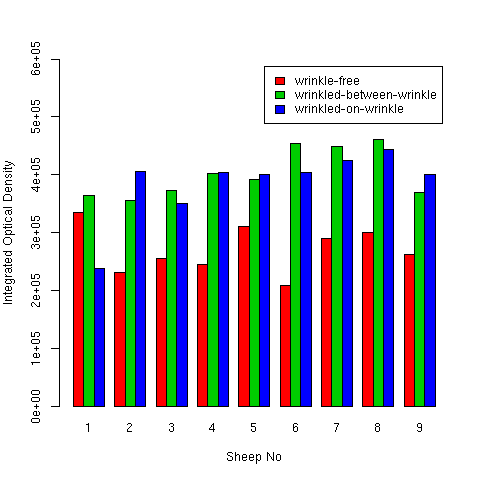
\includegraphics[scale=0.50]{t2f1odmeans.png}
% 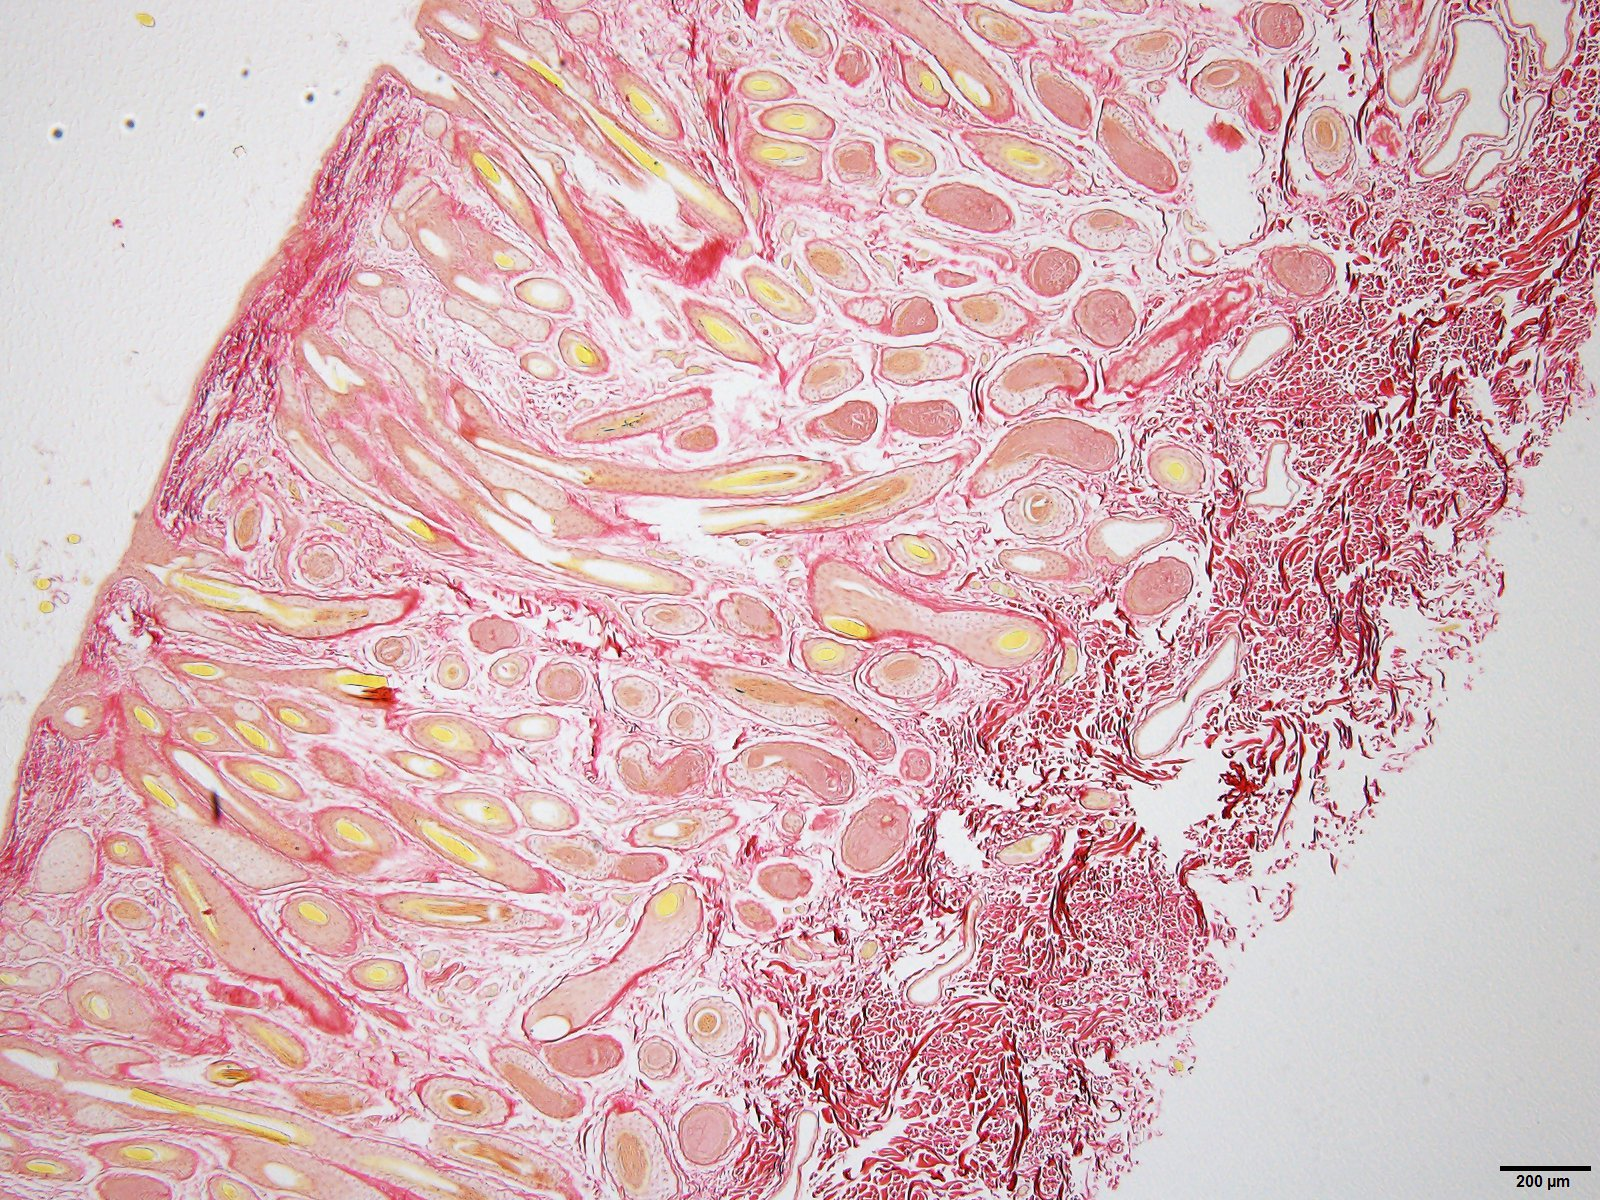
\includegraphics[width=1.0\textwidth]{w479-2-rigid.jpg}
  }
 \subfigure[Plate (ii) Flock No 2  of Trial 2]{
    \label{fig:redpixt2(ii)}
    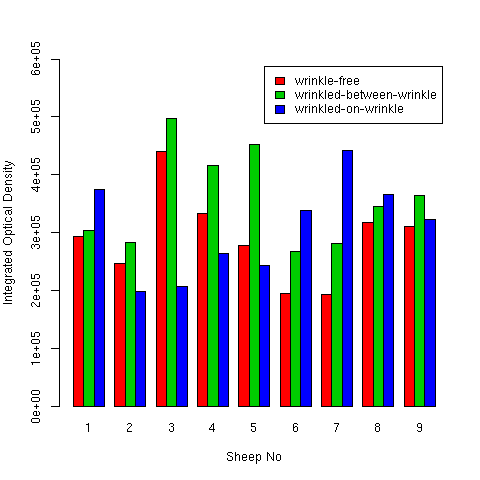
\includegraphics[scale=0.50]{t2f2odmeans.png}
  }
  \caption{Integrated optical density of the red images of sections stained with PSR for each of the nine sheep in each Flock of Trial 2, averaged over five microscope fields}
\vfill
  \label{fig:redpixt2}
\end{figure}

%\end{document}


These data are intended as a measure of the total amount of collagen tissue present in the microscope section at the position of the chosen field in the lower dermis.
The total number of pixels in an image taken with a 40x objective was 1920000, so one could scale these optical density sums to the average optical density of a pixel by dividing by 1920000. We chose not to do this scaling.
We can see that for Trial 1 the wrinkle-free sheep always had less collagen, except for those in Flock 4. In Trial 2  the wrinkle-free sheep always had less collagen than the between-wrinkle sample from the wrinkled sheep, but the on-wrinkle sample was more variable.

The significance of the differences apparent in Figure~\ref{fig:redpixt1} was tested by analysis of variance extracting terms for FlockNo, SkinType, and their interaction, as shown in Table~\ref{tab:redpixelt1aov}.
% latex table generated in R 3.4.2 by xtable 1.8-2 package
% Mon Jul 15 21:10:57 2019
\begin{table}[ht]
\centering
\caption{Analysis of variance of red pixel counts for Trial 1}
\label{tab:redpixelt1aov}
\begin{tabular}{lrrrrr}
  \hline
 & Df & Sum Sq & Mean Sq & F value & Pr($>$F) \\ 
  \hline
FlockNo & 1 & 48141986950.46 & 48141986950.46 & 9.87 & 0.0027 \\ 
  SkinType & 1 & 259320673232.61 & 259320673232.61 & 53.16 & 0.0000 \\ 
  FlockNo:SkinType & 1 & 26844676679.26 & 26844676679.26 & 5.50 & 0.0225 \\ 
  Residuals & 56 & 273170345102.88 & 4878041876.84 &  &  \\ 
   \hline
\end{tabular}
\end{table}


The residual term in Table~\ref{tab:redpixelt1aov} is the variation between randomly chosen Fields within a specimen, because there are no replicate sheep within each Flock:SkinType subclass. The difference between the wrinkled and wrinkle-free SkinTypes is shown to be significant but only at the 5\% level. The Flock differences are not significant, and there is an interaction.

The equivalent analysis of variance for Trial 2 (Figure~\ref{fig:redpixt2}) data is shown in Table~\ref{tab:redpixelt2aov}.
% latex table generated in R 3.4.2 by xtable 1.8-2 package
% Wed Jul 24 20:43:14 2019
\begin{table}[ht]
\centering

\caption{Analysis of variance of red pixel optical density sums for Trial 2}
\label{tab:redpixelt2aov}

\begin{tabular}{lrrrrr}
  \hline
 & Df & Sum Sq & Mean Sq & F value & Pr($>$F) \\ 
  \hline
FlockNo                  & 1 & 91548864255.47 & 91548864255.47 & 37.41 & 0.0000 \\ 
  SkinType                 & 1 & 412338258758.73 & 412338258758.73 & 168.48 & 0.0000 \\ 
  SampPos                  & 1 & 50325174039.48 & 50325174039.48 & 20.56 & 0.0000 \\ 
  FlockNo:SkinType         & 1 & 101676878442.96 & 101676878442.96 & 41.55 & 0.0000 \\ 
  FlockNo:SkinType:SheepNo & 49 & 1081769314333.64 & 22076924782.32 & 9.02 & 0.0000 \\ 
  Residuals                & 218 & 533522617623.69 & 2447351456.99 &  &  \\ 
   \hline
\end{tabular}
\end{table}


The difference between wrinkled and wrinkle-free SkinTypes is now shown to be highly significant. The Flock differences were not significant and there is a significant interaction of Flock with SkinType.  

 The on-wrinkle and between-wrinkle sampling positions within the wrinkled specimens were not significantly different . The on-wrinkle specimens actually had a lower integrated optical density than the between-wrinkle specimens indicating slightly {\em less} collagen on a wrinkle than between wrinkles.

There was also a significant amount of variation between sheep within the FlockNo and SkinType combinations. Sheep are much more variable than image Fields within a sheep, which is what the Residual term in Table~\ref{tab:redpixelt2aov} represents. In this analysis the Sheep term is the error term for all terms above it in the analysis of variance table, whereas in Trial 1 there was no sheep replication and we were forced to use the FlockNo:SkinType term as the error. This explains why the SkinType differences were less significant in Trial 1. 

The actual means and their standard deviations for integrated optical density for both Trial 1 and Trial 2 are shown in Table~\ref{tab:redpixelodmeans}
%\documentclass{article}
%\usepackage{lscape}
%\begin{document}

\begin{table}[htp]
\centering
\caption{Means and standard errors for integrated red pixel optical density of wrinkled and wrinkle-free sheep in Trial 1 and Trial 2}
\label{tab:redpixelodmeans}
\vspace{0.1in}
\begin{tabular}{|p{0.5in}|p{0.6in}|p{1.0in}|p{1.0in}|p{1.0in}|}  \hline
     Trial & Parameter &  Wrinkle-free  &  Wrinkled (between-wrinkle) & Wrinkled (on-wrinkle)  \\ 
\hline
  1  & Mean &   83748        &   215232   &       \\
  1  & Standard deviation &   47535      &    98720   &  \\ \hline
  2  & Mean &   280851       &   380427    &  347170   \\ 
  2  & Standard deviation &    70609     &  75988  &  96787 \\ \hline
\end{tabular}
\end{table}

%\end{document}

We see that the wrinkle-free sheep actually have a very low amount of collagen in Trial 1. This is probably because the Trial 1 sheep were selected from SRS-Merino stud flocks and those chosen as wrinkle-free were likely to be extreme examples of wrinkle-free sheep, of a type not found in normal Merino flocks. 

The Trial 2 sheep are the opposite. These were from commercial flocks, and here the wrinkled sheep ( either the on-wrinkle or between wrinkle specimens) had a higher amount of collagen than the wrinkled sheep from Trial 1. Again, this simply reflects the fact that more extreme wrinkled sheep were available for selection in rial 2. 

The standard deviations were greater for wrinkled sheep, and greater for on-wrinkle than between-wrinkle specimens. Apparently wrinkled skins are more variable, at least in their collagen density. We did not test whether these differences in standard deviation were significant.

The data and analyses show that there is more collagen in the lower dermis of wrinkled sheep than wrinkle-free sheep.  The actual size of the difference varied from 2.5 x in Trial 1 to 1.4 x in Trial 2. 
Within wrinkled sheep there was no difference in amount of collagen between samples taken on a wrinkle or between wrinkles.




\subsubsection{Spatial location and structure of collagen}
We have shown that there is more collagen in wrinkled sheep. We need to look and see if it occupies the same part of the dermis. We also need to investigate whether the arrangement of collagen fibres varies.

The best images for these purposes were taken with a 10x objective. Figure~\ref{fig:he10x} shows images of layers 2 and 3 in specimens from two sheep, one being wrinkled (a between-wrinkle specimen) and one being wrinkle-free.
%\documentclass{article}
%\usepackage{graphicx,subfigure}
%\usepackage{caption,rotating}
%\begin{document}

\begin{figure}[p]
\centering
 \subfigure[Plate (i) Sheep 3453 Wrinkled]{
    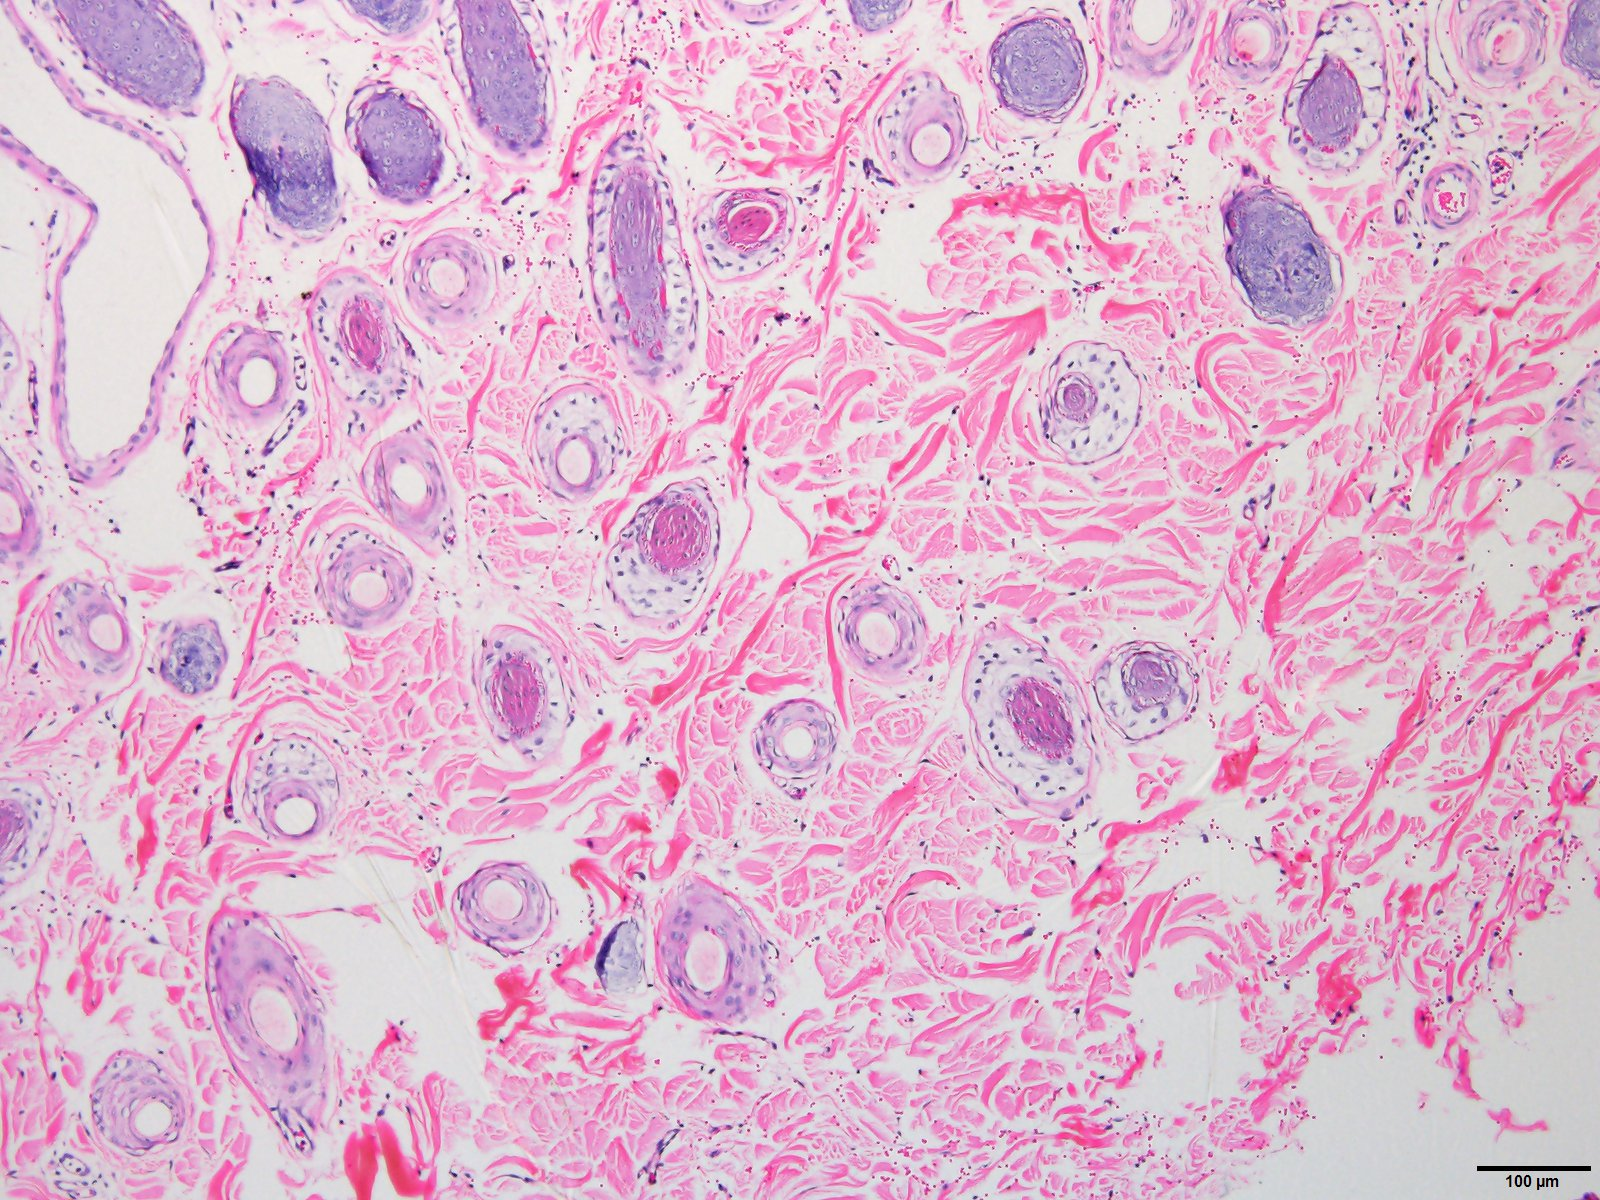
\includegraphics[scale=0.20]{3453_btwn_wrinkle_10x.jpg}
% 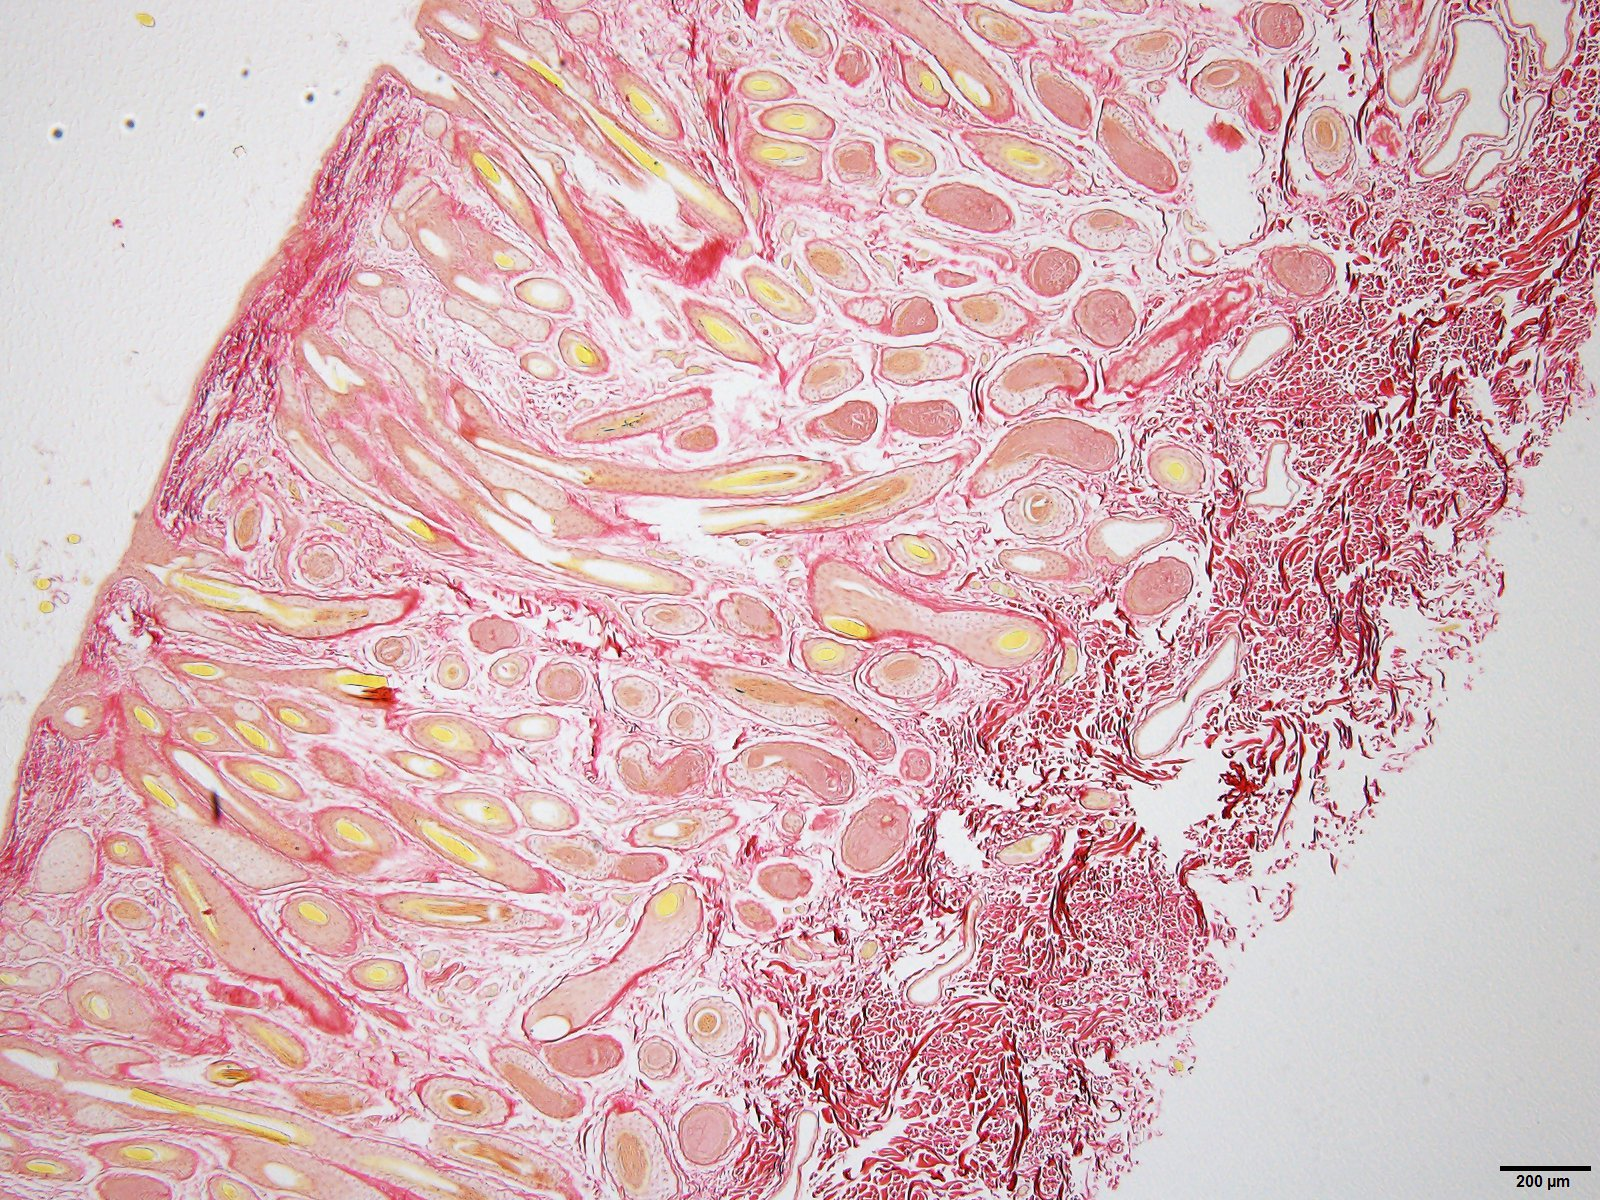
\includegraphics[width=1.0\textwidth]{w479-2-rigid.jpg}
  }
 \subfigure[Plate (ii) Sheep 3458 Wrinkle-free]{
    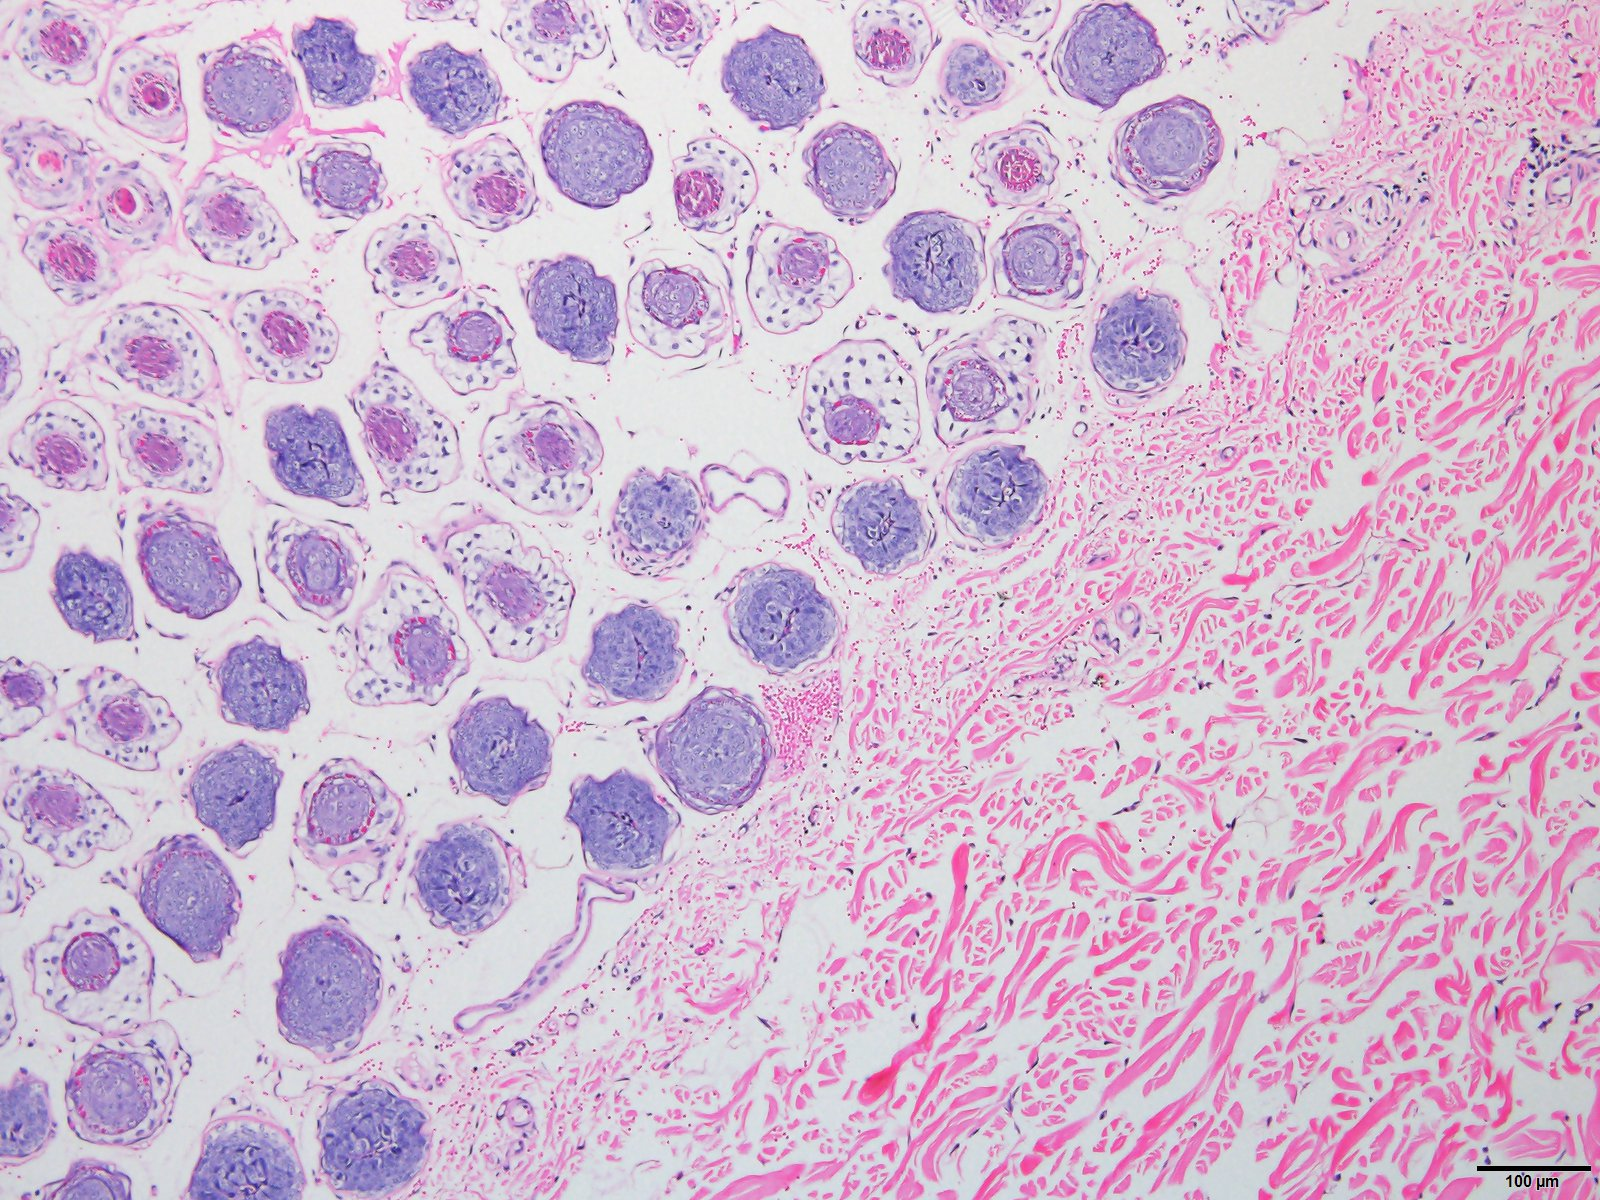
\includegraphics[scale=0.20]{3458_smooth_10x.jpg}
  }
  \caption{Vertical sections from a wrinkled (i) and a wrinkle-free (ii)  sheep from Trial 2 flock 1 stained with H-E. and viewed with a 10x objective. }
\vfill
  \label{fig:he10x}
\end{figure}

%\end{document}


The most obvious difference is that in the wrinkled sheep specimen the collagen extends up into the follicular region, there being conspicuous amounts of collagen in and around the follicle bulbs. In the wrinkle-free sheep there is very little amount of collagen in amongst the follicle bulbs, and the collagen immediately below the bulbs is fine structured and presumably of a reticular type. 

There is also a difference in structure. In the wrinkled sheep there are large pieces of very dense collagen ( judging by the intensity of staining)  in the lower dermis, and amongst the follicles. These large entities are presumably bundles of collagen fibrils. In the wrinkle-free sheep there are some dense pieces of collagen ( more further down in the dermis) but these are not as dense and not as large and not as numerous as in the wrinkled specimen. If we look back to the PSR stained images of Figure~\ref{fig:psr40x}, these observations are confirmed. We must note that we are viewing thin (4 micron) sections. For bundles of collagen to show as large continuous areas in these sections they must align with the direction of sectioning. Hence we see some fibre bundles that have been sectioned across, and these show as small entities, and some that have been sectioned along and these show as large entities. There are fewer large entities in the wrinkle-free specimens in both Figures~\ref{fig:psr40x} and ~\ref{fig:he10x}. This difference is even discernable in the images viewed with a 4x objective shown in Figure~\ref{fig:trial24xhe}

We were not able to quantify these observations. The examples we have shown are from Trial 2, but the differences were consistent across both trials.

\subsubsection{Type of collagen}
The types of collagen relevant to skin are
\begin{description}
\item[Type I] or {\em hard} collagen forms thick bundles of eosin staining fibres. Is present in tendons, ligaments, and scar tissue. It binds things together.
\item[Type III] or {\em soft or reticulate} collagen forms thin separate  eosin staining fibres which crosslink to form a fine mesh network supporting soft tissues.  It often occurs with Type I.
\end{description}
Both types occur together in skin. The strength, elasticity  and flexibility of skin come from the presence of collagen and elastin fibres, and presumably variations in these properties would derive from variations in the amounts and proportions of these types. For example changes in skin with ageing are partly a result of reduction in Type I collagen.

One can distinguish the two Types of collagen simply from the size of the fibrils. For example in  the PSR stained images of Figure~\ref{fig:psr40x} the wrinkled specimen clearly has large bundles of fibrils and therefore a considerable amount of Type I collagen. The wrinkle-free specimen, however has fewer bundled fibrils, and lots of thin individual fibrils. This is also quite obvious in the H-E stained sections of Figures~\ref{fig:he10x} and ~\ref{fig:trial24xhe}.

There is a somewhat contentious technique referred to in the Methods section, which uses polarized light microscopy to attempt to differentiate Type I from Type III collagen.  The collagen fibres are birefringent and it is asserted that they show coloured red, orange, yellow, or green on order of thickness of the bundles of fibrils. Thus, red and orange would be likely to indicate Type I collagen, and yellow and green would be likely to indicate Type III collagen.

Figure~\ref{fig:polar} shows two polarized light images under a 4x objective comparing a wrinkled sheep with a wrinkle-free sheep.
%\documentclass{article}
%\usepackage{graphicx,subfigure}
%\usepackage{caption,rotating}
%\begin{document}

\begin{figure}[p]
\centering
 \subfigure[Plate (i) Sheep w479 Wrinkled]{
%   \label{fig:trial1he(i)}
    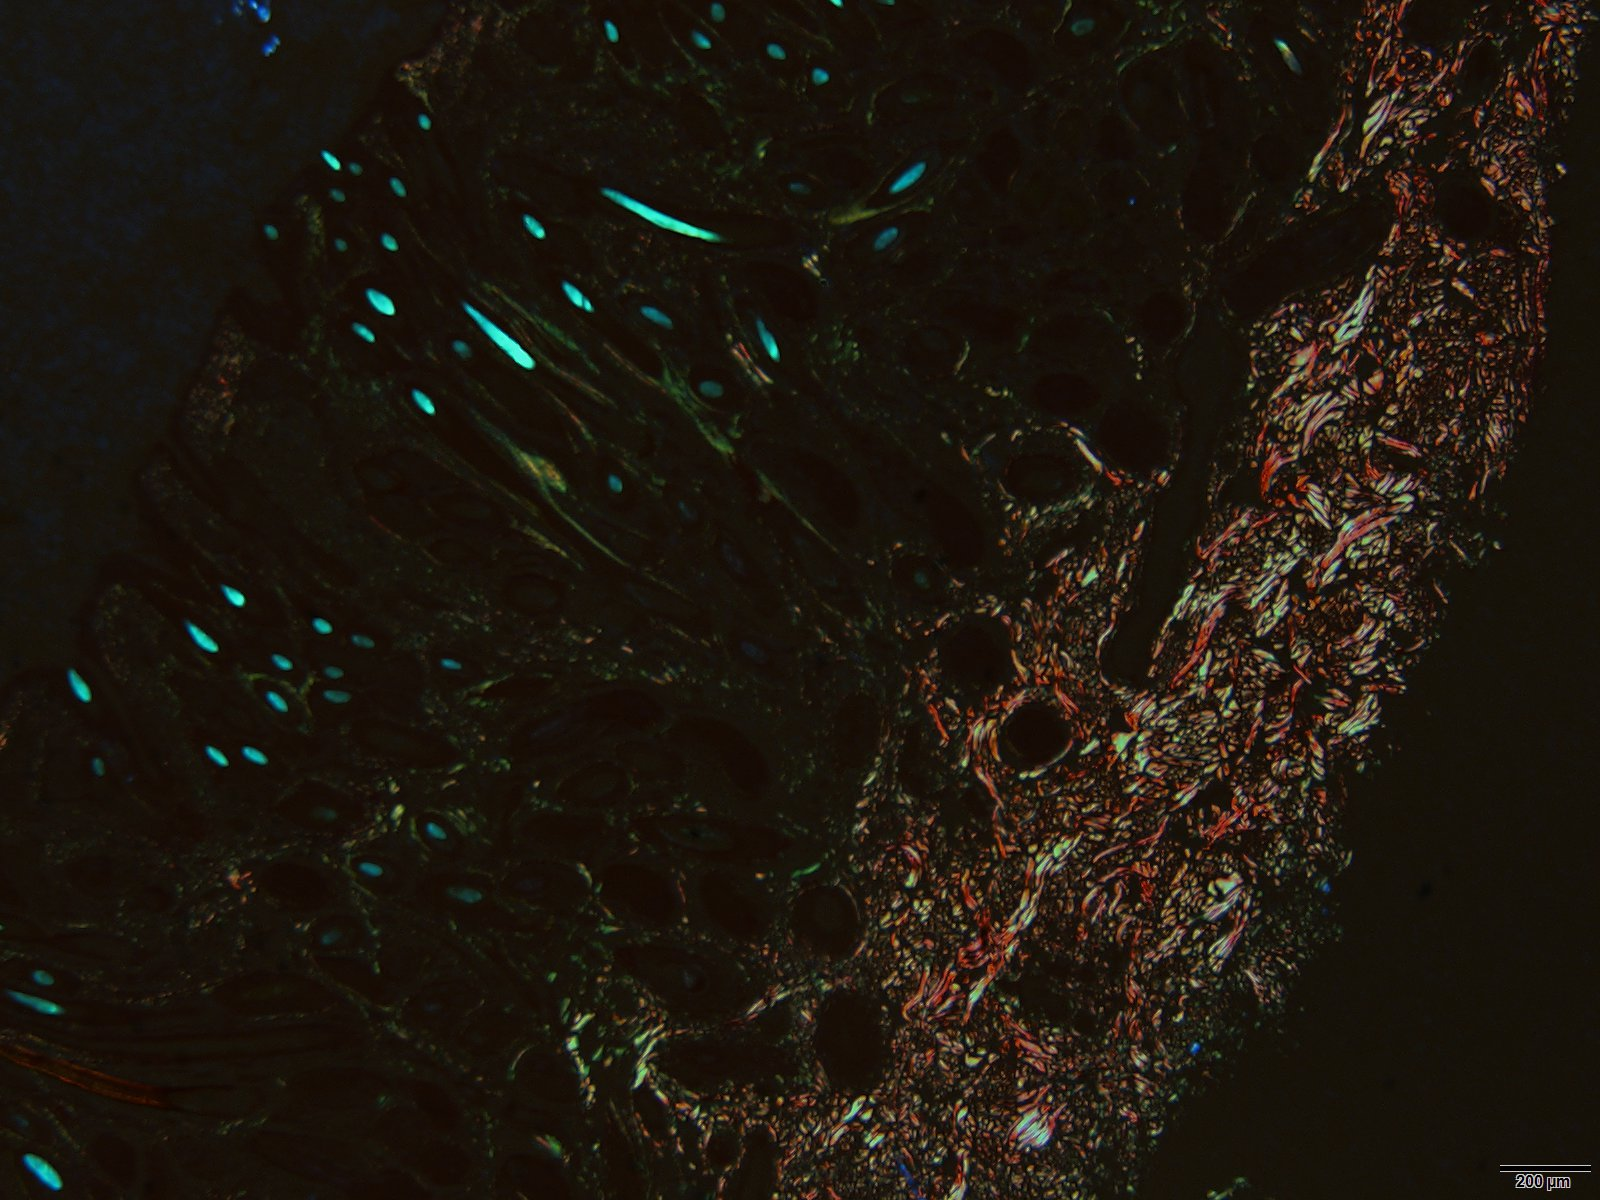
\includegraphics[scale=0.20]{w479-2_rigid_PSR_stain_polarised.jpg}
% 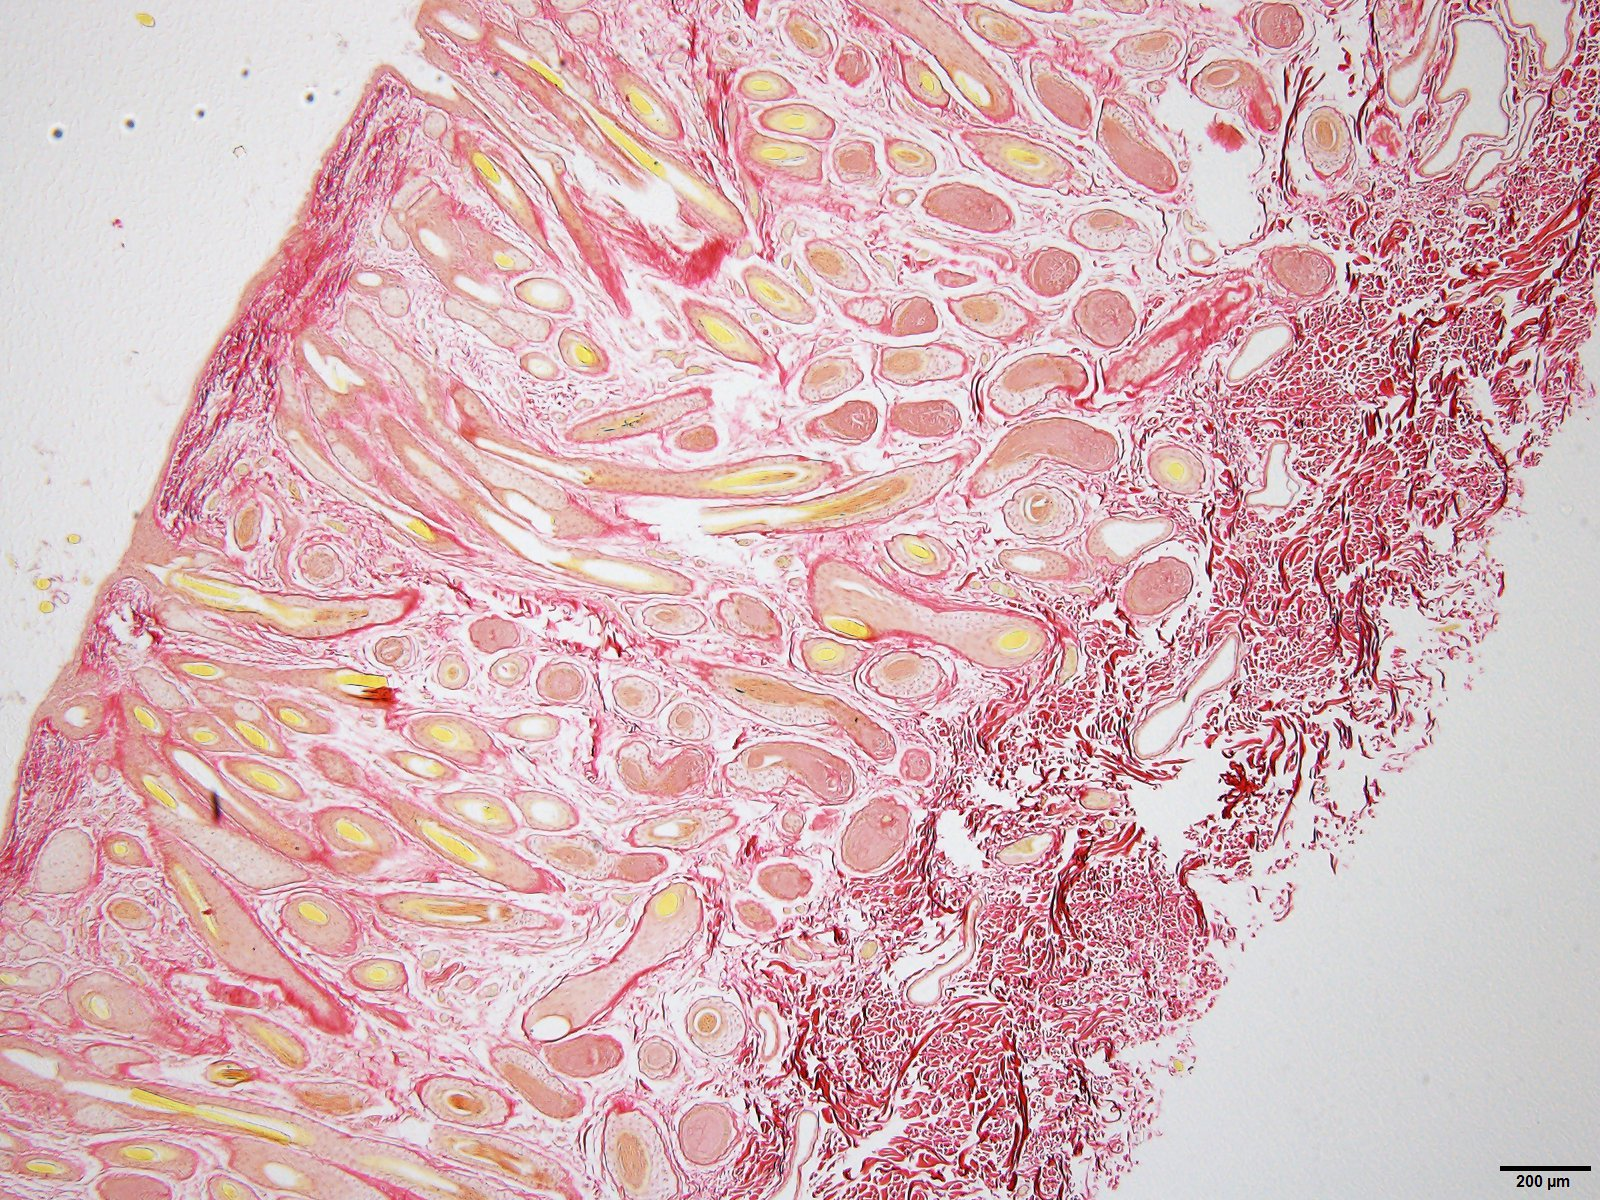
\includegraphics[width=1.0\textwidth]{w479-2-rigid.jpg}
  }
 \subfigure[Plate (ii) Sheep w490 Wrinkle-free]{
%   \label{fig:trial1he(ii)}
    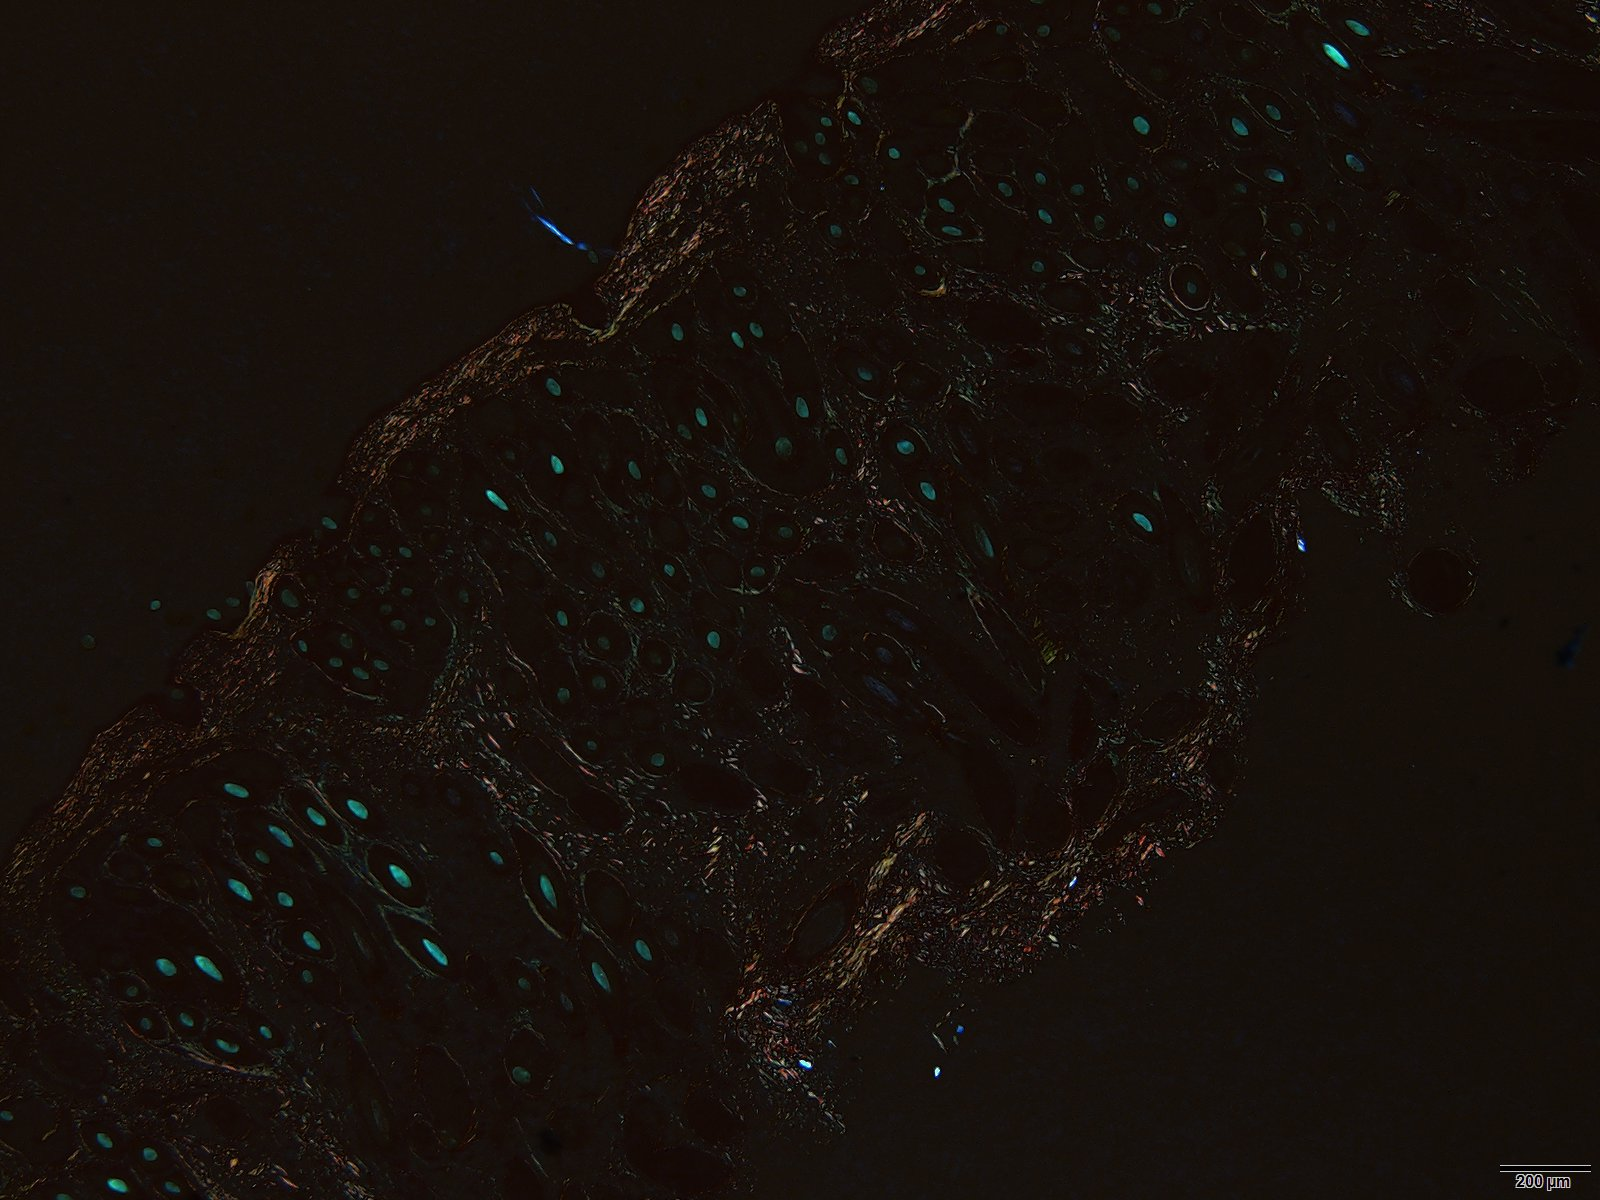
\includegraphics[scale=0.20]{w490-2_supple_PSR_stain_polarised.jpg}
  }
  \caption{Vertical sections from a wrinkled (i) and a wrinkle-free (ii)  sheep from Trial 1 flock 2 stained with PSR and examined with polarised light and a 4x objective. }
\vfill
  \label{fig:polar}
\end{figure}

%\end{document}


The same sections viewed under normal bright field microscopy are shown in Figure~\ref{fig:nopolar}. 
%\documentclass{article}
%\usepackage{graphicx,subfigure}
%\usepackage{caption,rotating}
%\begin{document}

\begin{figure}[p]
\centering
 \subfigure[Plate (i) Sheep w479 Wrinkled]{
    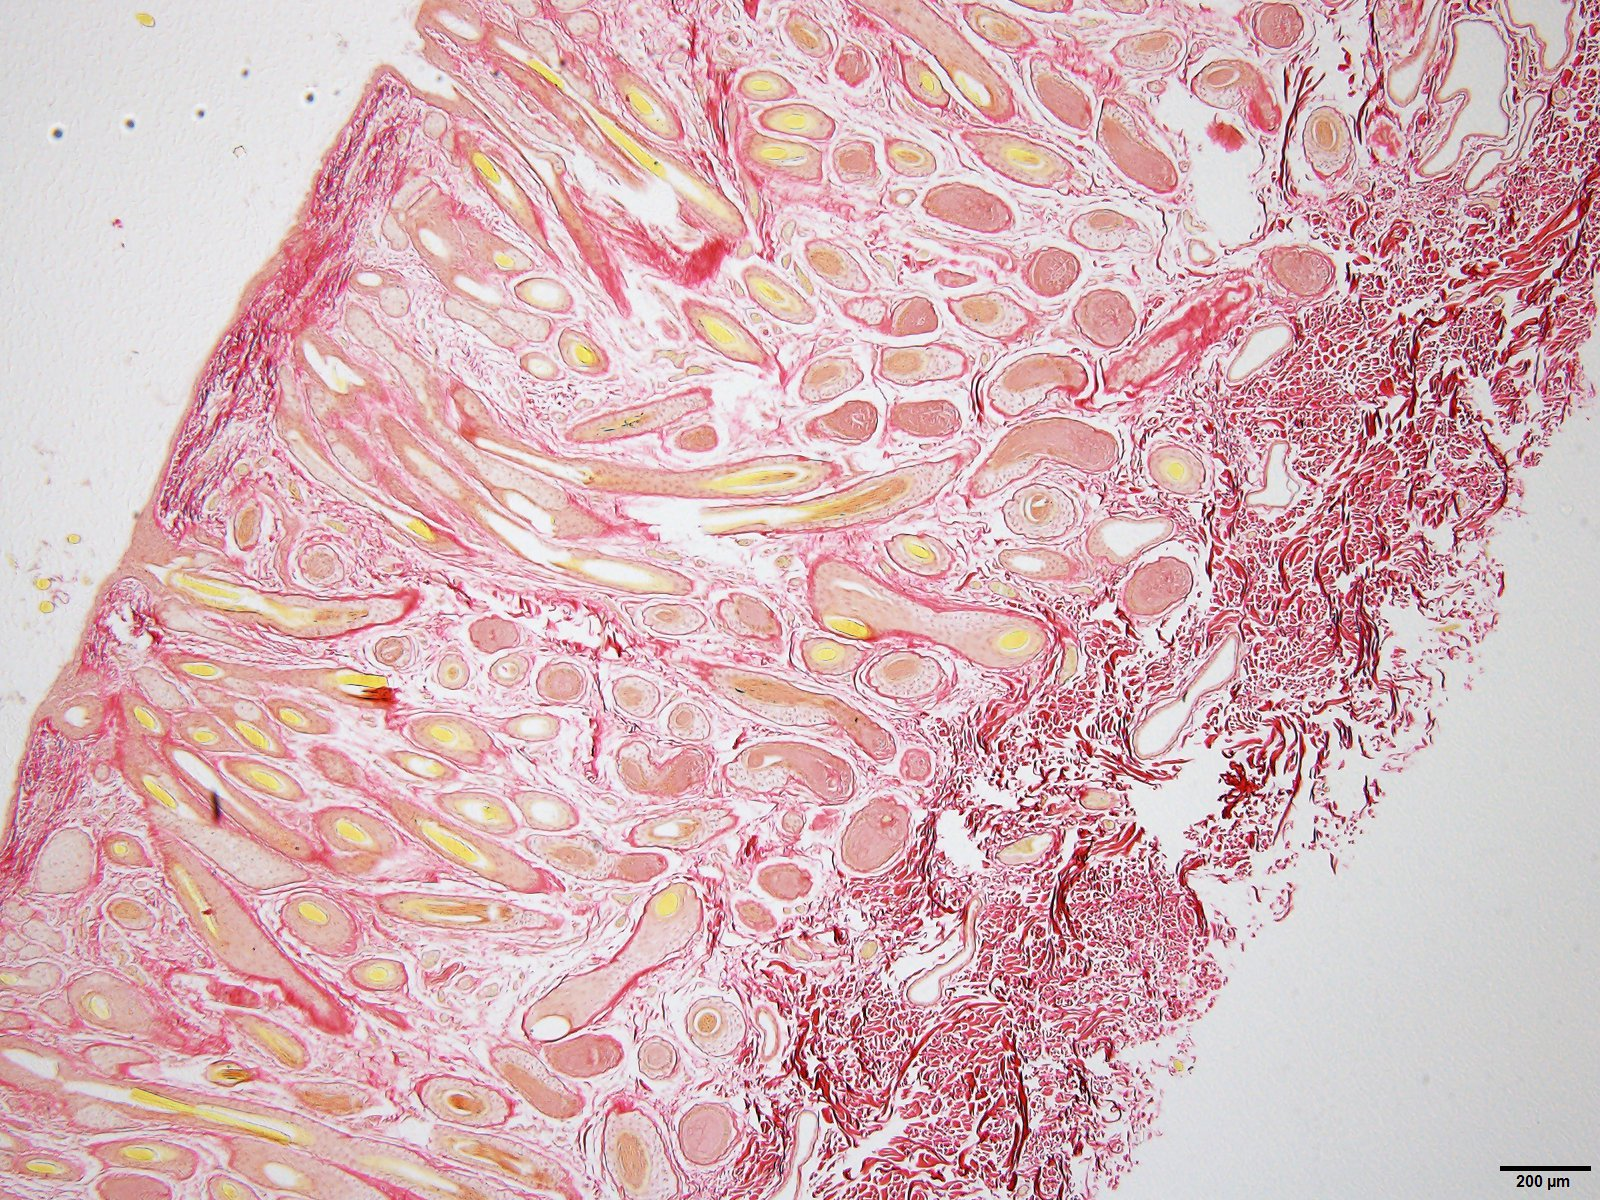
\includegraphics[scale=0.20]{w479-2-rigid.jpg}
  }
 \subfigure[Plate (ii) Sheep w490 Wrinkle-free]{
    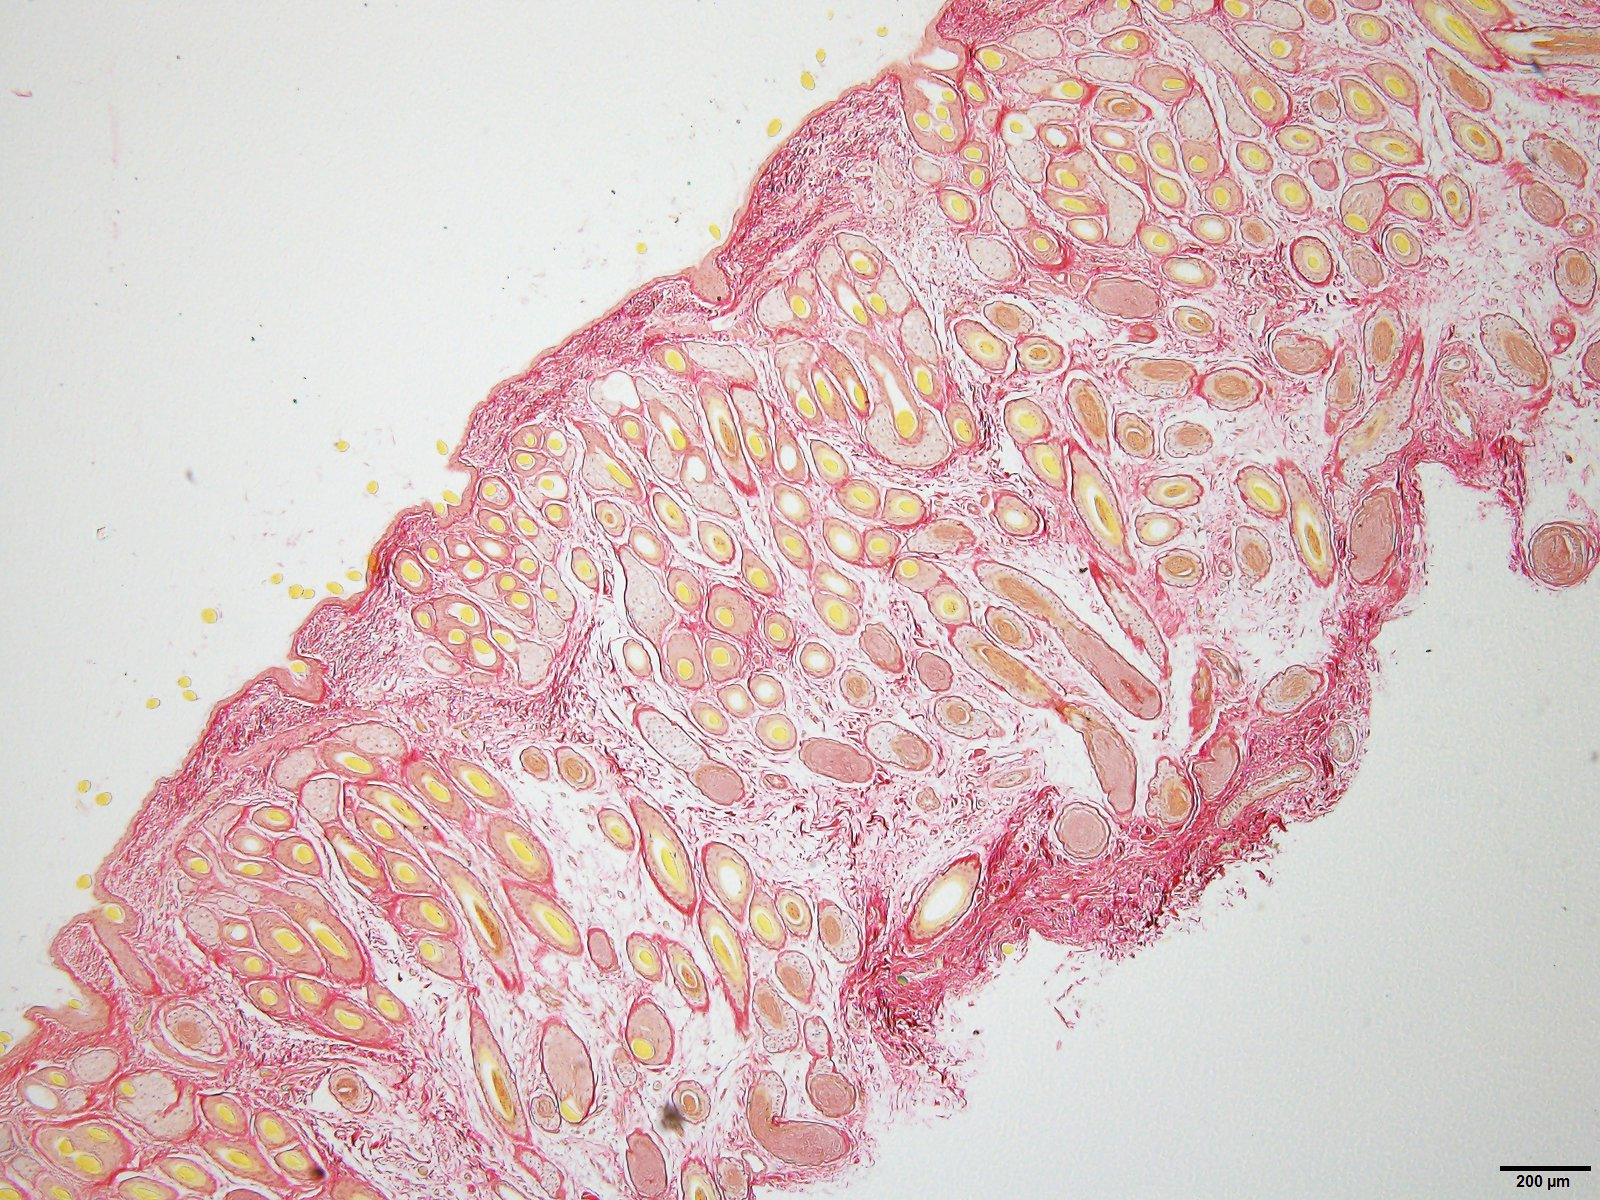
\includegraphics[scale=0.20]{w490-2-supple.jpg}
  }
  \caption{Vertical sections from a wrinkled (i) and a wrinkle-free (ii)  sheep from Trial 1 flock 2 stained with PSR and examined with a 4x objective. These are the same two sections as shown with polarised light in Figure~\ref{fig:polar}. }
\vfill
  \label{fig:nopolar}
\end{figure}

%\end{document}


It can be seen that while both the wrinkled and wrinkle-free specimens have some lower dermal collagen ( stained red with PSR stain in Figure~\ref{fig:nopolar}), only the wrinkled specimen shows orange/red birefringence under polarised light (Figure~\ref{fig:polar}). 

So, there is the proof that wrinkled sheep do not just have more collagen, but the extra collagen is Type I (hard). The wrinkle-free sheep apparently has only Type III (reticular) collagen. This confirms what we concluded in the previous section from looking at the size of collagen fibre bundles.

\subsubsection{Fibroblasts}
The dermal cells which produce collagen fibrils are called {\em fibroblasts} or mesenchymal stem cells.  Fibroblasts also produce reticular fibres, and the pre-papilla cells that aggregate during follicle formation.

Some differences were observed in the fibroblasts in wrinkled and wrinkle-free sheep. We are only able to report Dr Watt's observation
\begin{quote}
"The dermal fibroblasts in the wrinkled sheep appear to be mature, slender fibroblasts (fibrocytes) with dark staining nuclei whereas wrinkle-free sheep have immature, plumb fibroblasts with pale staining nuclei. The density of fibrobasts in the wrinkled sheep also appears to be higher than in wrinkle-free sheep"
\end{quote}

Further observations would be required to confirm this. If correct it would mean that the dermal collagen of wrinkled sheep was under more active development at the time of sampling.

\subsection{Follicle characteristics}
A number of follicle attributes seem to differ between wrinkled and wrinkle-free sheep. These are documented below

\subsubsection{Follicle curvature scores}
Follicle curvature scores were available for Trial 1. The scores for each sheep are shown on Table~\ref{tab:curv}
%\documentclass{article}
%\usepackage{lscape}
%\begin{document}

\begin{table}[htp]
\centering
\caption{Follicle curvature  scores Flocks 1 to 5 of Trial 1}
\label{tab:curv}
\vspace{0.1in}
\begin{tabular}{|p{0.6in}|p{0.6in}|p{0.8in}|p{0.8in}|}  \hline
     Flock No. & Sheep No.  &  Skin Type & Follicle Curvature Score  \\ 
\hline
  1 & W206 & Wrinkle-free & 3  \\
  1 & W205 & Wrinkled     & 6  \\
  2 & W490 & Wrinkle-free & 4  \\
  2 & W479 & Wrinkled     & 6  \\
  3 & W555 & Wrinkle-free & 3  \\
  3 & W547 & Wrinkled     & 7  \\
  4 & W567 & Wrinkle-free & 3  \\
  4 & W558 & Wrinkled     & 3  \\
  5 & W283 & Wrinkle-free & 2  \\
  5 & W290 & Wrinkled     & 7  \\ \hline
\end{tabular}
\end{table}

%\end{document}

In each case except for Flock 4, the wrinkle-free sheep had a lower follicle curvature score than the wrinkled sheep.

An analysis of variance of these scores is given in Table~\ref{tab:curvaov}
% latex table generated in R 3.4.2 by xtable 1.8-2 package
% Wed Jul 17 20:21:12 2019
\begin{table}[ht]
\centering
\caption{Analysis of variance of follicle curvature score for Trial 1 data}
\label{tab:curvaov}
\begin{tabular}{lrrrrr}
  \hline
 & Df & Sum Sq & Mean Sq & F value & Pr($>$F) \\ 
  \hline
FlockNo & 4 & 5.4 & 1.35 & 0.73 & 0.616 \\ 
  SkinType & 1 & 19.60 & 19.60 & 11.43 & 0.0117 \\ 
  Residuals & 7 & 12.00 & 1.71 &  &  \\ 
   \hline
\end{tabular}
\end{table}


This shows that the difference between wrinkle-free and wrinkled sheep was significant at the 1 percent level.

\subsubsection{Follicle curvature measurements}
Follicle curvature measurements were made for Trial 2. There is a document detailing measurement methods and their statistical analysis available in Watts and Jackson (2018)~\cite{watt:18}. 

Here we present only a summary of the results. Table~\ref{tab:curvmeasmeans} shows means for follicle depth, straight length of the follicle, curved length of the follicle and radius of curvature. 
%\documentclass{article}
%\usepackage{lscape}
%\usepackage{tablefootnote}
%\begin{document}

\begin{table}[ht]
\centering
\caption{Means for follicle measurements separately for each Flock and each Skintype for Trial 2}
\label{tab:curvmeasmeans}
\vspace{0.1in}
\begin{tabular}{|p{0.5in}|p{0.6in}|p{0.6in}|p{0.6in}|p{0.6in}|p{0.6in}|} \hline
  Flock & Skin.type & Folldepth & Straightlen & Curvlen  & Radcurv\\   
    \hline
  1 & wrinkle-free & 1.579 & 1.827 & 1.839 & 6.97  \\ 
  2 & wrinkle-free & 1.721 & 1.846 & 1.854 & 8.99  \\ 
  1 & wrinkled & 1.972 & 2.136 & 2.222 & 2.92 \\ 
  2 & wrinkled & 1.833 & 1.925 & 2.035 & 2.15  \\ 
   \hline
\end{tabular}
\end{table}

%\end{document}



All four measurements differed between wrinkled and wrinkle-free sheep,and the differencess were significant for all four traits.
There is a comprehensive analysis of these follicle curvature measurements in Watts and Jackson(2018)~\cite{watt:18}. 
The important result is that the wrinkled sheep had a much smaller radius of curvature, meaning that the follicles were more curved in wrinkled sheep. This confirms the subjective follicle curvature scores, which were for Flock 1 of Trial 2 3.8 for wrinkled sheep and 1.7 for wrinkle-free sheep, and for Flock 2 of Trial 2 5.1 for wrinkled sheep and 2.7 for wrinkle-free sheep (means of 9 sheep in each case).

 The follicles of wrinkled sheep were also slightly deeper and longer. 

\subsubsection{Follicle density and S/P ratio}
For Trial 2, some further measurements of the follicle and fibre characteristics were available, and are shown in Table~\ref{tab:follmeas}
%\documentclass{article}
%\usepackage{lscape}
%\usepackage{tablefootnote}
%\begin{document}

\begin{table}[ht]
\centering
\caption{Means for follicle density and fibre diameter measurements separately for each Flock and each Skintype for Trial 2}
\label{tab:follmeas}
\vspace{0.1in}
\begin{tabular}{|p{0.5in}|p{0.6in}|p{0.6in}|p{0.6in}|p{0.6in}|p{0.6in}|} \hline
  Flock & Skin.type & Follicle density & S/P ratio & Dp  & Ds\\   
    \hline
  1 & wrinkle-free & 83.9 & 27.8 & 16.4 & 18.4  \\ 
  2 & wrinkle-free & 94.9 & 27.8 & 17.7 & 18.4  \\ 
  1 & wrinkled & 76.7 & 21.8 & 18.8 & 20.7 \\ 
  2 & wrinkled & 66.8 & 22.6 & 20.5 & 20.7  \\ 
   \hline
\end{tabular}
\end{table}

%\end{document}



Wrinkled sheep had lower follicle density, lower S/P ratio, and coarser primary and secondary fibres.
\begin{verbatim}
Awaiting raw data so can complete aov for these traits.
 Need to show differences are significant.
\end{verbatim}

\subsubsection{Follicular degeneration}
Dr Watts saw evidence of follicle degeneration in wrinkled sheep. His statement was
\begin{quote}
"  I am happy that there is not only follicular distortion caused by collagen but also follicular degeration.  I can see evidence of bent follicle bulbs right at the tip of where the follicles are curving more or less at right angles.  I can also see in these affected sheep, the wrinkly skinned ones, that the follicle bulb cells are becoming vacuolated ie. undergoing cellular degeneration. The fibre defects we are encountering appear to be the consequence of this follicle degeneration."
\end{quote}

There are no measurements to support this statement. The fibre defects referred to are fibre naps. 

\subsection{Wrinkle patterns over the body}
The small {\em pin} wrinkles which all Merinos have do not seem to make any pattern. They are uniform across the body of the sheep. We are considering here the large folds which develop ( in wrinkled sheep only) after birth and up to maturity. These form a very consistent pattern which was documented by Carter(1943)~\cite{cart:43}. Dr Carter actually named each fold, and recognized that each fold along the body of the sheep was associated with successive vertebrae along the spine. The pattern is therefore very regular from sheep to sheep. Only the size of folds varies, not the pattern.

Figure~\ref{fig:sheep} shows a photograph of two Merino ewes, with and without wrinkle. 
%\documentclass{article}
%\usepackage{graphicx,subfigure}
%\begin{document}

\begin{figure}[!h]
  \centering
  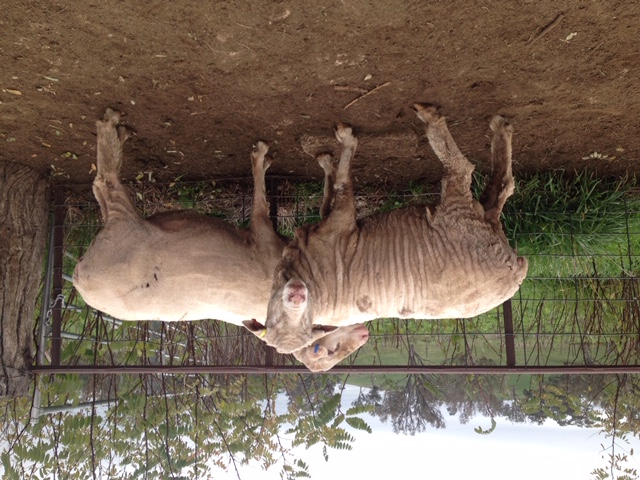
\includegraphics[width=1.0\textwidth,angle=180]{IMG_0322.JPG}
  \caption{Two Merino ewes from Flock 1 of Trial 2, one wrinkled and one wrinkle-free}
  \label{fig:sheep}
\end{figure}

%\end{document}


The wrinkled sheep in Figure~\ref{fig:sheep} is a good example of the pattern to which we refer.  Each fold runs vertically from dorsal to ventral positions, and there are approximately the same number of folds as vertebrae. So each fold appears to mark the position one dermatome area of skin, with the main nerve from the spine running either under the fold or between the folds. We do not know the spatial relationship between folds and nerve channels, but is appears to be a one-to-one relation.


\clearpage
\section{Discussion}
We have established the following from observations on adult Merino sheep
\begin{itemize}
\item wrinkled sheep have skin which is more supple and more compressible
\item wrinkled sheep have more collagen in the lower dermis
\item wrinkled sheep have more Type I collagen in the lower dermis
\item in wrinkled sheep the collagen in the lower dermis extends upwards around the follicle bulbs into the upper dermis
\item there is no difference in collagen between sites on a wrinkle or between wrinkles within wrinkled sheep
\item wrinkled sheep have more highly curved follicles
\item wrinkled sheep have lower follicle density and lower S/P ratio as adults
\item wrinkled sheep have coarser fibre diameters, both primary and secondary fibres as adults
\end{itemize}

In addition we know the following from other published work
\begin{itemize}
\item pin wrinkles are small and are present at birth and remain into adulthood. They are mainly a characteristic of Merino sheep
\item large folds grow in size as the sheep matures, but can be visible at birth. They are also mainly a characteristic of Merino sheep.
\item large folds consist of epidermis, papillary dermis, and lower or reticular dermis, but not the muscle and fat layers 
\item collagen is present in the foetal dermis from about day 80, ie at about the same time as when the secondary derived follicles are forming
\item collagen in the dermis gradually becomes more Type I as the sheep matures 
\item developing follicles in the foetus can be seen to be curved, before they grow a fibre
\end{itemize}


\clearpage
\begin{thebibliography}{99}

\bibitem{bogo:40}
 Bogolyubsky S.N. (1940) cited by Fraser A.S and Short B.F. (1960) The Biology of the Fleece. Animal Research Laboratories Technical Paper No 3. CSIRO Melbourne 1960.

\bibitem{brow:68}
Brown, G.H., and Turner, Helen Newton. (1968) Response to selection in Australian Merino sheep. II. Estimates of phenotypic and genetic parameters for some production traits in Merino ewes and an analysis of the possible effects of selection on them. Aust. J. Agric. Res. 19:303-22

\bibitem{cart:43}
Carter H.B. (1943) Studies in the biology of the skin and fleece of sheep. 1. The development and general histology of the follicle group in the skin of the Merino. 2. The use of tanned sheepskin in the study of follicle population density. 3. Notes on the arrangement, nomenclature, and variation of skin folds and wrinkles in the Merino. C.S.I.R. Bulletin No 164, Melbourne, 1943

\bibitem{fras:60}
Fraser A.S and Short B.F. (1960) The Biology of the Fleece. Animal Research Laboratories Technical Paper No 3. CSIRO Melbourne 1960.

\bibitem{gord:08}
Gordon-Thompson, C., Botto, S.A., Cam, G.R., and Moore, G.P.H. (2008) Notch pathway gene expression and wool follicle cell fates. Aust. J. Exp. Agric. 48(5) 648-656

\bibitem{jack:75}
Jackson, N., Nay, T, and Turner, Helen Newton (1975) Response to selection in Australian Merino sheep. VII Phenotypic and genetic parameters for some wool follicle characteristics and their correlation with wool and body traits. Aust. J. Agric. Res. 26:937-57

\bibitem{jack:15}
Jackson, N. (2015) Genetic relationship betweeen skin and wool traits in Merino sheep. Incomplete manuscript.

\bibitem{jack:17}
Jackson, N. (2017) Genetics of primary and secondary fibre diameters and densities in Merino sheep. URL https://github.com/nevillejackson/atavistic-sheep/mev-rewrite/supplementary/genetic-parameters/psparam.pdf

\bibitem{jack:17a}
Jackson, N. (2017) Genetic relationship between skin and wool traits in Merino sheep. Part I Responses to selection ans estimates of genetic parameters. URL https://github.com/nevillejackson/Fleece-genetics/tree/master/skinandfleeceparameters/ab3220/skinwool1.pdf

\bibitem{jack:18}
Jackson, N. and Watts, J.E. (2018) Does follicle development affect the spatial layout of sheep skin? URL https://github.com/nevillejackson/Fleece-biology/tree/master/skinspace/skinspace.pdf

\bibitem{jack:90}
Jackson, N., Maddocks, I.G., Lax, J., Moore, G.P.M. and Watts, J.E. (1990) Merino Evolution, Skin Characteristics, and Fleece Quality. URL https://github.com/nevillejackson/atavistic-sheep/mev/evol.pdf 

\bibitem{jack:17b}
Jackson, N. and Watts, J.E. (2017) What is known about the genetics of wrinkle score in Merino sheep? URL https://github.com/nevillejackson/Fleece-genetics/wrinkle/wrinkle.pdf

\bibitem{junq:79}
Junqueira L.C.U., Bignolas G., Brentani R.R. Picrosirius staining plus polarization microscopy, a specific method for collagen detection in tissue sections. Histochem J 1979; 11, 447-455

\bibitem{kier:99}
Kiernan, J.A.(1999) Histological and Histochemical Methods: Theory and Practice. Ed 3. Butterworth Heinemann, Oxford, UK

\bibitem{knig:93}
Knight, K.R., Lepore, D.A., Horne, R.S., Ritz, M., Kumta, S. and O'Brian, B.M. (1993) Collagen content of uninjured skin and scar tissue in foetal and adult sheep. Int. J. Exp. Pathol. 74(6):583-591

\bibitem{latt:14}
Lattouf, R., Younes, P., Lutomski, D., Naaman, N., Godeau, G., Senni, K. and Changotade, S. (2014  Picrosirius red staining: a useful tool to appraise collagen networks in normal and pathological tissues. J. Histochem. Cytochem. 62(10): 751-758

\bibitem{madd:88}
Maddocks, I.G. and Jackson, N. (1988) Structural studies of sheep, cattle, and goat skin. CSIRO, Division of Aimal Production, Sydney.

\bibitem{ment:80}
Menton, D.N. and Hess, R.A. (1980) The ultrastructure of collagen in the dermis of tight-skin (Tsk) mutant mice. The Journal of Investigative Dermatology 74:139-147

\bibitem{mitc:84}
Mitchell, T.W. et al (1984) Some physical and mechanical properties of sheep akin with a comparison of "thick" and "thin" skins. Wool Technology and Sheep Breeding, Vol XXXII, No IV, 200-206

\bibitem{moor:89}
Moore G.P.M., Jackson, N., and Lax, J. (1989) Evidence of a unique developmental mechanism specifying both wool follicle density and fibre size in sheep selected for single skin and fleece characters. Genet. Res. Camb. 53:57-62

\bibitem{moor:98}
Moore, G.P.M., Jackson, N., Isaacs, K., and Brown, G (1998) J. Theoretical Biology 191:87-94

\bibitem{nay:66}
Nay, T. (1966) Wool follicle arrangement and vascular pattern in the Australian Merino. Aust. J. Agric. Res. 17:797-805

\bibitem{rprog:13}
R Core Team (2013). R: A language and environment for statistical
  computing. R Foundation for Statistical Computing, Vienna, Austria.
  ISBN 3-900051-07-0, URL http://www.R-project.org/.

\bibitem{ryde:68}
Ryder, M.L. and Stevenson, S.K.(1968) Wool Growth. Academic Press, London.

\bibitem{sedd:31}
Seddon, H.R., Belschner, H.G. and Mulhearn, C.R. (1931)  Studies on cutaneous myiasis of sheep. Sew South Walse Department of Agriculture, Science Bulletin No 37, 1931

\bibitem{turn:56} 
Turner, Helen Newton (1956) Anim. Breed. Abstr. 24:87-118

\bibitem{turn:58}
Turner, Helen Newton(1958) Aust. J. Agric. Res. 9:521-52

\bibitem{turn:53}
Turner, Helen Newton, Hayman, R.H., Riches, J.H., Roberts, N.F., and Wilson, L.T. (1953) Physical definition of sheep and their fleece for breeding and husbandry studies: with particular reference to Merino sheep. CSIRO Div. Anim. Hlth. Prod. Div. Rept. No. 4 (Ser SW-2 mimeo)

\bibitem{turn:68}
Turner, H.N., Dolling, C.H.S., and Kennedy, J.F. (1968) Response to selection in Australian Merino sheep. I. Selection for high clean wool weight with a ceiling on fibre diameter and degree of wrinkle. Response in wool and body characteristics. Aust. J. agric. Res. 19:79-112

\bibitem{turn:70}
Turner, Helen Newton, Brooker M.G. and Dolling, C.H.S (1970) Response to selection in Australian Merino sheep. III Single character selection for high and low values of wool weight and its components. Aust.J.Agric.Res. 21:955-84

\bibitem{watt:18}
Watts, J.E., Jackson, N. (2018) Follicle depth, straight length, and curved length in plain and wrinkly sheep. URL https://github.com/nevillejackson/SRS-Merino/blob/master/supplementary/depthandcurv/depthandcurv.pdf

\bibitem{watt:17}
Watts, J.E., Jackson, N., and Ferguson, K.A. (2017) Improvements in fleece weight weight and wool quality of Merino sheep selected visually for high fibre density and length. URL https://github.com/nevillejackson/SRS-Merino/Paper\_2\_Revised\_10\_November\_2017.docx 

\bibitem{xavi:03}
Xavier, S.P., Gordon-Thomson, C. Wynn, P.C., McCullagh, P., Thomson, P.C., Tomkins, L., Mason, R.S., and Moore, G.P.M.(2003) Evidence that Notch and Delta expressions have a role in dermal condensate aggregation during wool follicle initiation. Experimental Dermatology, 22:656-681

\end{thebibliography}
\end{document}
